\chapter{Results and Discussion}
\label{cha:results}

\section{Numerical Tests in an 2D Toy Potential}
\label{sec:2D}
As a simple test to check all ABM methods a single particle in the two-dimensional potential $U_2$ (eq.~\ref{eq:U2}) was considered.
By performing a 2D to 2D mapping in the absence of any dimensionality reduction, the analytical PMF and free energy difference is given by
\begin{equation}
  \begin{split}
    A(x,y)&=U_2(x,y) \\
    \Delta A_{A\to B} &= 0
  \end{split}
\end{equation}
The convergence of numerical PMFs and free energy differences to the analytical result was computed with different adaptive biasing schemes (MtD, WTM, ABF, eABF and WTM-eABF) from 5~ns trajectories.
Note that all adaptive biasing methods depend on a different set of parameters.
Their convergence can therefore only be compared qualitatively.
A detailed analysis of the impact of the choice of parameters will be given in the following section.
Parameters applied in this section and resulting PMFs after 1, 3 and 5~ns are given in the appendix.
Figure~\ref{fig:conv 2D} shows the convergence of the PMF and corresponding estimate for the free energy difference and figure~\ref{fig:error 2D} gives remaining absolute local errors at the end of all simulations.

In an unbiased simulation the system stays trapped in one metastable state.
This is a example of quasi-nonergodic behavior, where simple time averages of MD trajectories do not converge to the correct ensemble average in a reasonable time frame.
Because only a small region of CV space is explored the free energy difference $\Delta A_{A\to B}$ is highly overestimated.

All adaptive biasing methods reduce the metastability significantly and enable uniform sampling of both states.
In MtD/WTM simulations the PMF is given by a superposition of Gaussian hills, which are deposited linearly over time and fill both minima consecutively.
For this particular set of parameters no full convergence is reached in 5~ns.
Regions with high free energy at the margins remain unexplored due to incomplete filling of the PMF with Gaussians and the obtained PMFs deviate from the analytic result by about 20~\%.
However, this is no concern for the calculation of free energy differences as long as the PMF is estimated accurately in the remaining area.
WTM makes use of this insight by scaling down the Gaussian height over time, which reduces fluctuations and absolute errors of the PMF compared to MtD.
% The fraction of the PMF that will be compensated by Gaussian hills is given a priori by $\frac{\Delta T}{T+\Delta T}$.
% For $\Delta T=2000$~K this leads to a factor of 0.87.
After 4~ns the free energy difference $\Delta A_{A\to B}$ obtained from WTM therefore converges safely towards 0~kJ/mol.
\begin{figure}[H]
   \centering
   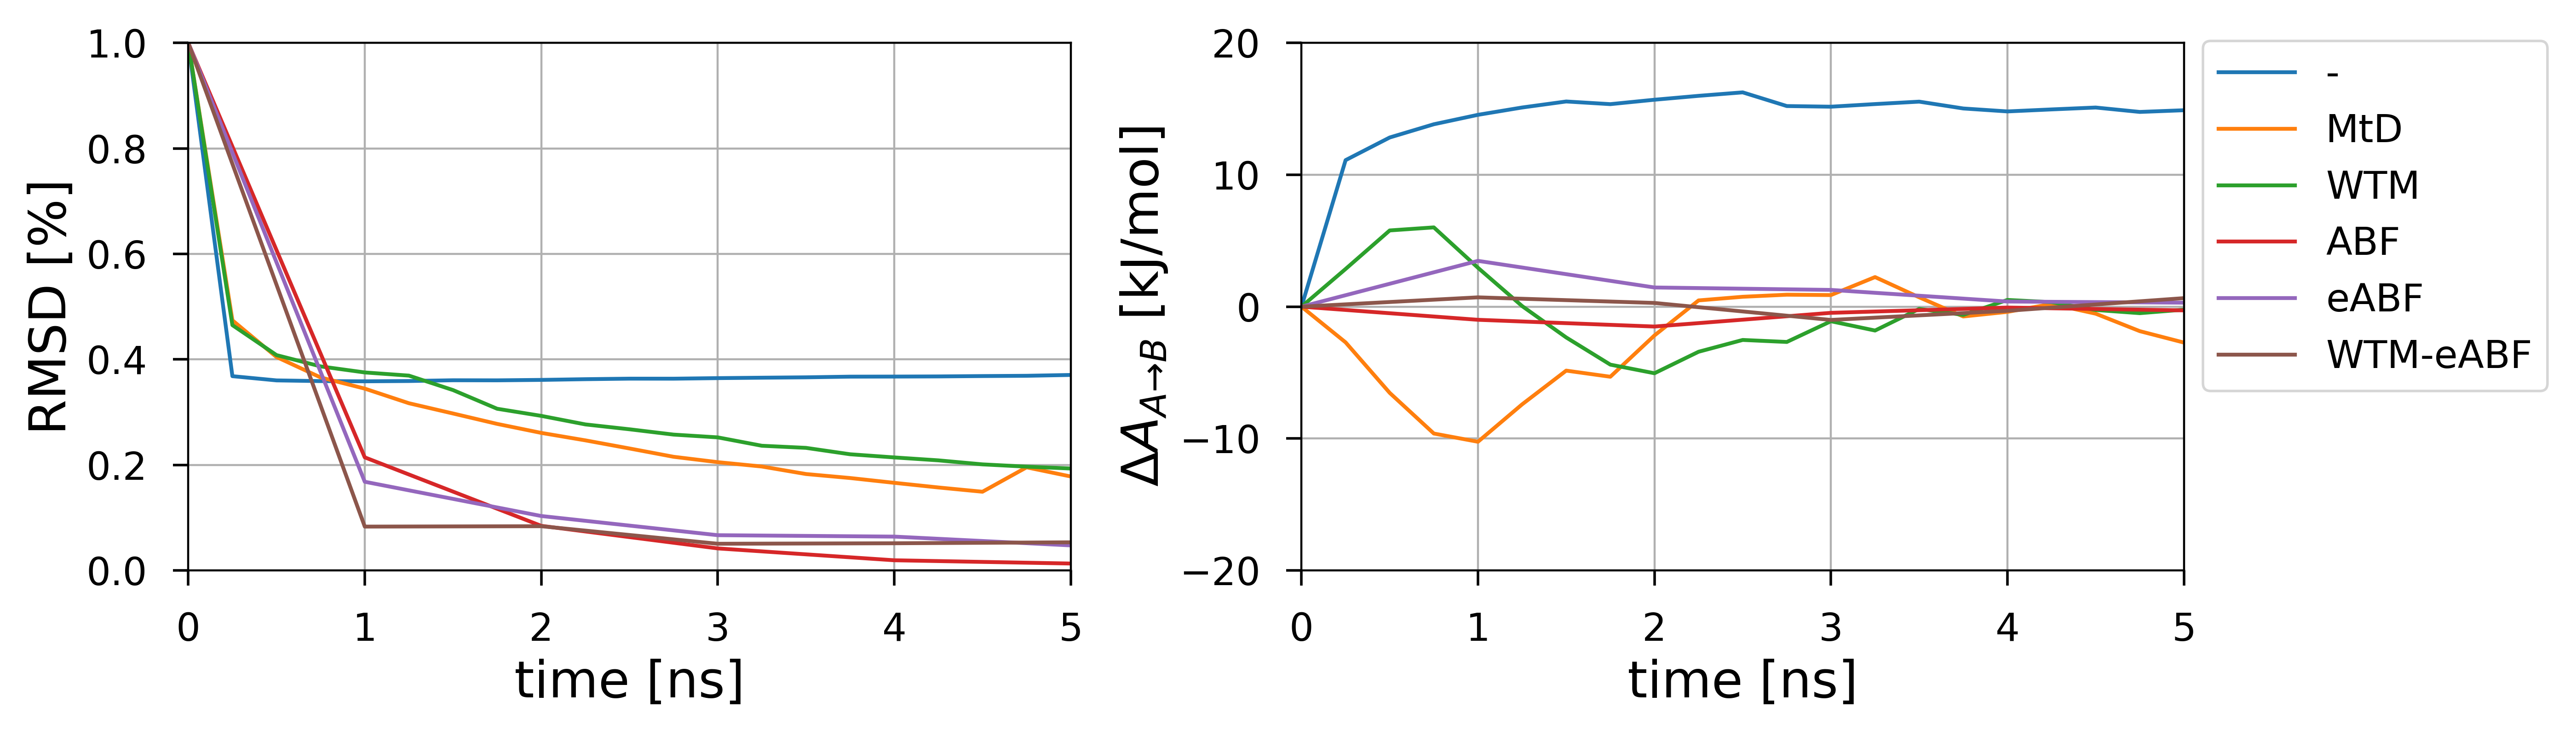
\includegraphics[width=0.99\textwidth]{bilder/test_2D/conv}
   \caption{Convergence of free energy calculations with different adaptive biasing methods for a 2D to 2D mapping of toy potential $U_2$. On the right the RMSD between the analytical and numerical PMF is given over the course of 5~ns trajectories. On the right the development of free energy differences $\Delta A_{A\to B}$ given by eq.~\ref{eq:free energy diff} is shown. Both metastable states are separated by the transition barrier located along the line $0.25x+y$. Therefore $A$ includes all states with $x>-4y$ and $B$ all states with $x<-4y$, respectively.}
 \label{fig:conv 2D}%
\end{figure}
\begin{figure}[H]
  \centering
  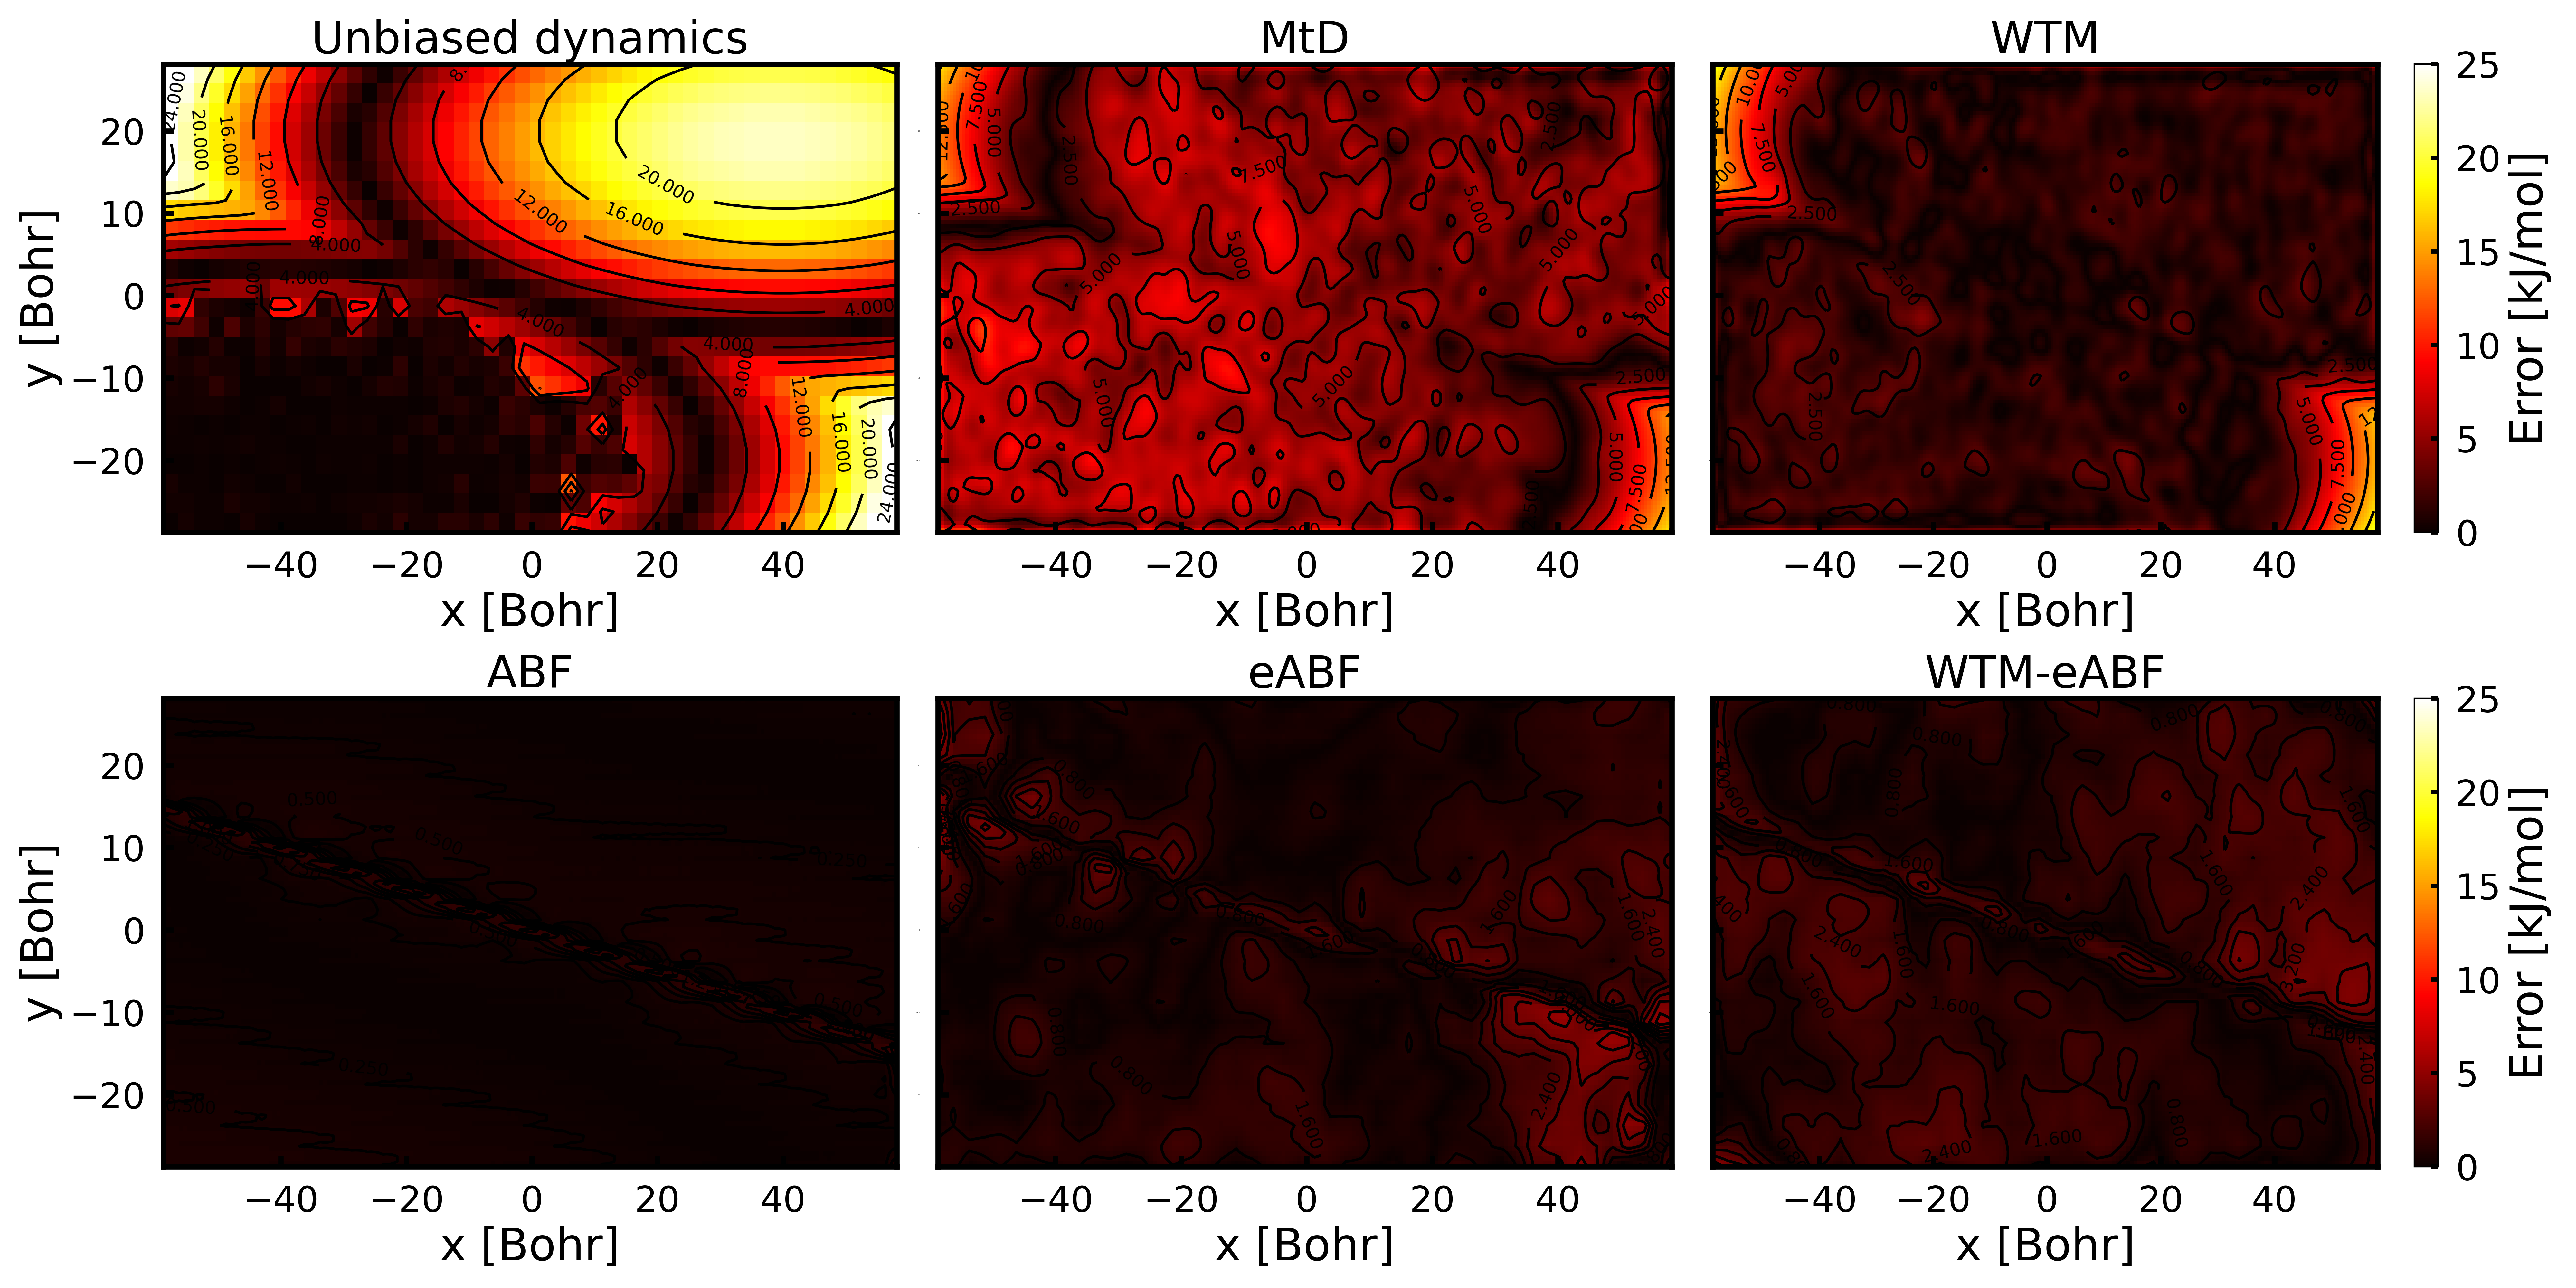
\includegraphics[width=0.99\textwidth]{bilder/test_2D/error_5ns}
  \caption{Heat maps of the absolute difference between the analytic and numerical PMFs. Numerical PMFs are obtained from 5~ns MD trajectories at 300~K.}
\label{fig:error 2D}%
\end{figure}
With ABF after 3~ns the potential is mapped almost perfectly with maximum local errors below 1~kJ/mol.
Also the RMSD of the PMF and free energy difference $\Delta A_{A\to B}$ converges rigorously to the analytic results.
For this toy example ABF force samples are simply given by the gradient of the analytical potential.
The variance of force samples, which is only introduced by the finite bin width, is therefore small and convergence of the ABF force in individual bins is reached almost instantly.
Even faster exploration of the PMF is only hindered by the ramp function, which is not strictly necessary for this example, but still applied to provide a more realistic test case for real chemical applications.
PMFs are obtained by thermodynamic integration of ABF forces with the FEM method, as shown in figure~\ref{fig:ti}.
Convergence of the FEM method is reached reliably in 100 iterations by minimization of eq.~\ref{eq:RMSD} with the BFGS algorithm.
After the minimization small errors of 0.2~kJ/(molBohr$^2$) remain at the transition barrier, where the gradients of $U_2$ change rapidly.
This error can be further reduced by using a smaller bin width.

By estimating the thermodynamic force over an extended-system fluctuations of force samples in eABF or WTM-eABF simulations depend on the harmonic force constant of the coupling of the fictitious to the physical particle.
In this toy example this increases the noise of the mean force estimate compared to ABF, which is visible in the thermodynamic integration of the eABF forces shown in figure~\ref{fig:ti}.
Especially at the beginning of a simulation, when free energy gradients obtained from CZAR are not yet full converged, minimization of the error function yields relatively high final errors.
The resulting PMF shows small fluctuations of up to 2~kJ/mol for both methods and convergence to the true PMF is reached with a final PMF RMSD of about 2~\%.
However, with eABF convergence of the PMF RMSD is reached as fast as with ABF and WTM-eABF gives an additional significant speed up.
With WTM-eABF the estimate for $\Delta A_{A\to B}$ stays between $-1$ and $1$~kJ/mol over the hole simulations.
This indicates that no state is preferentially sampled throughout the simulation and the entire PMF is evenly visited.
\begin{figure}[H]
  \centering
  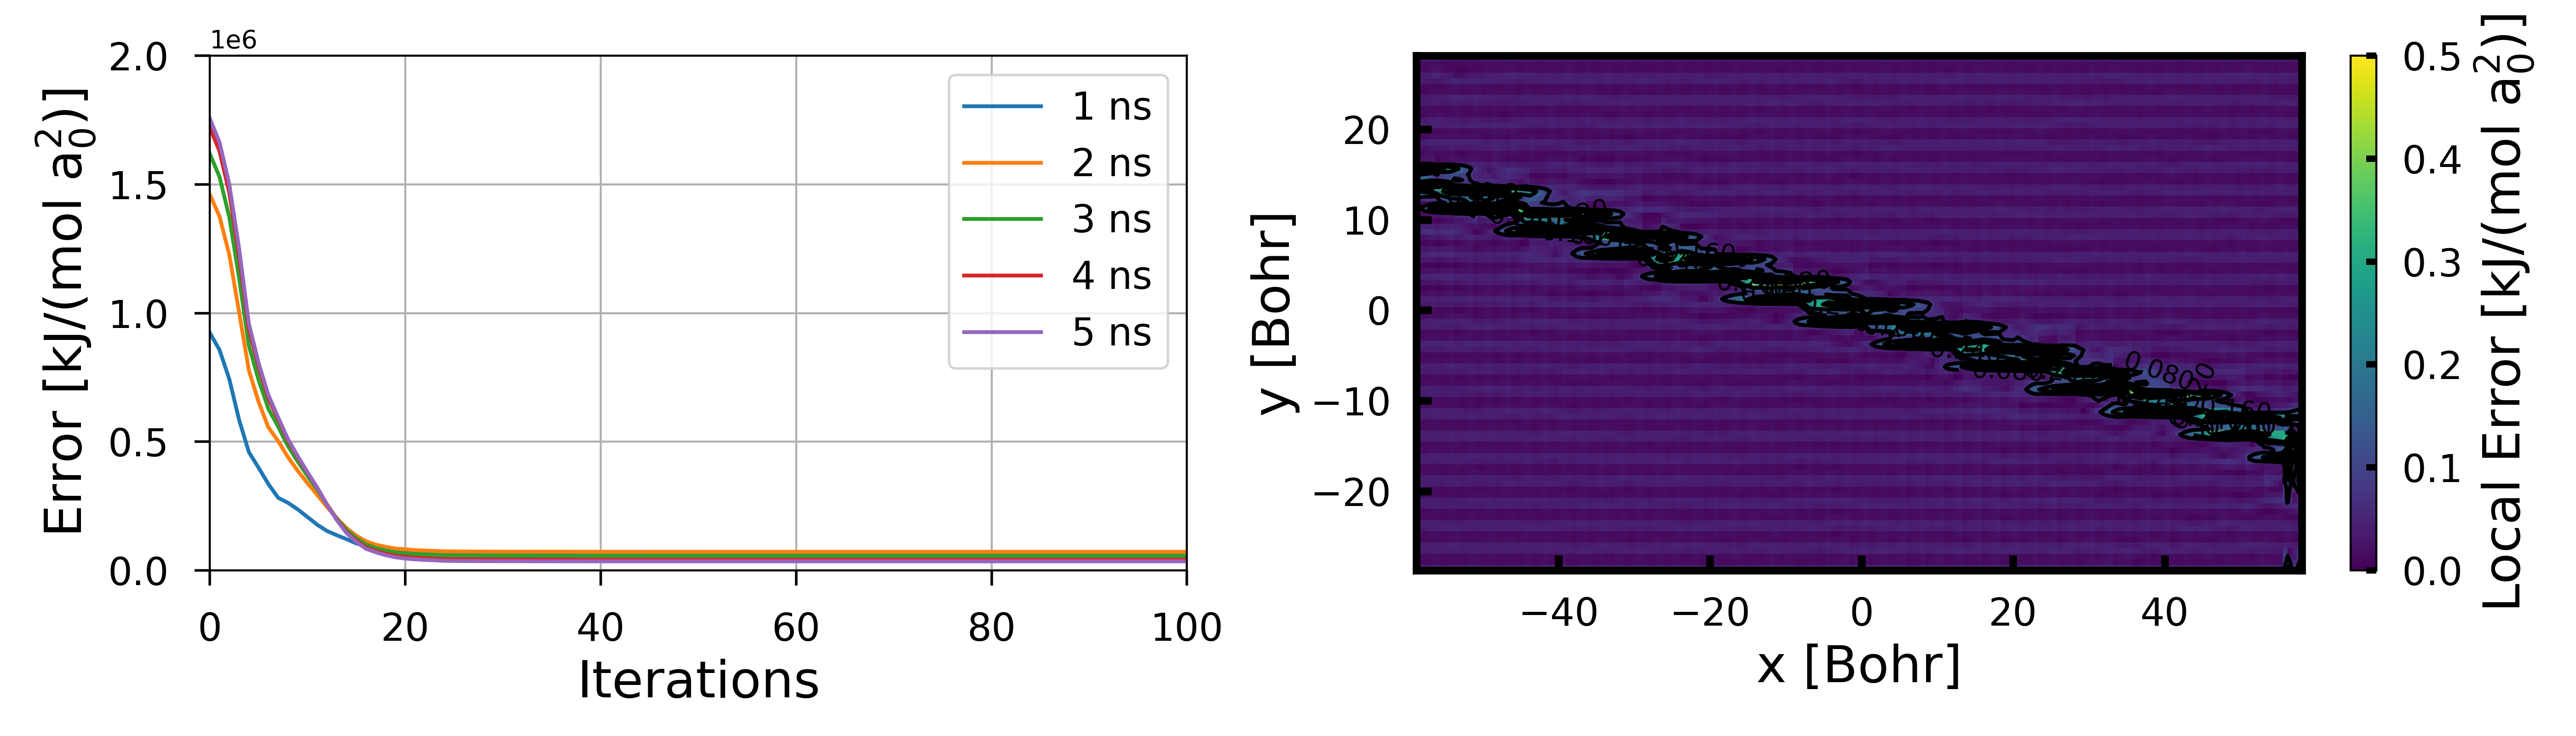
\includegraphics[width=0.99\textwidth]{bilder/test_2D/ti}
  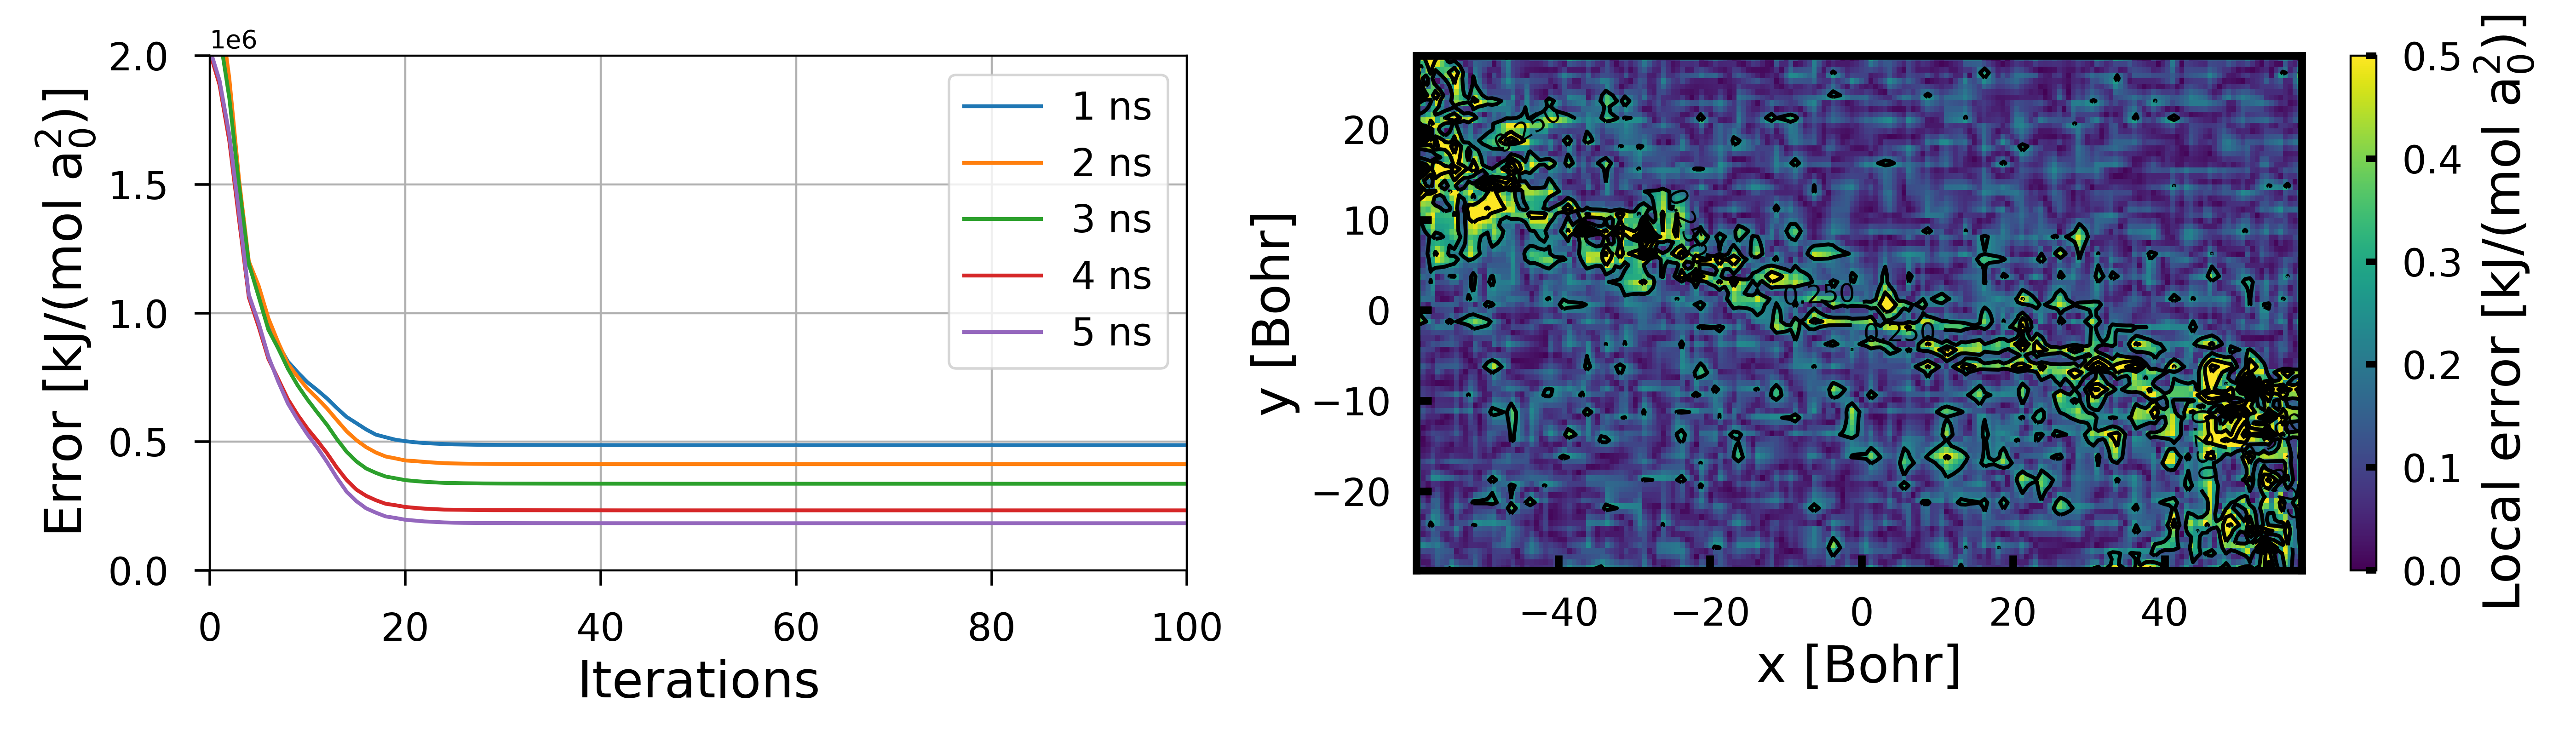
\includegraphics[width=0.99\textwidth]{bilder/test_2D/ti_eABF}
  \caption{
  FEM integration of thermodynamic forces obtained from ABF and eABF simulations.
  On the left the convergence of the minimization of equation~\ref{eq:FEM} with the BFGS algorithm is given for force estimates at different time steps. On the right the mean local error of optimized B-splines to free energy gradients for the x- and y-direction obtained from 5~ns trajectories is shown.}
\label{fig:ti}%
\end{figure}
Overall, all adaptive biasing methods enhance sampling of the PMF significantly.
Especially accurate PMFs are obtained from ABF based methods (ABF, eABF and WTM-eABF), which enable uniform exploration even for the highest free energy regions at the margins.
In the following sections this methods will be discussed in further detail for the application to a real chemical system with special focus on the influence of input parameters on the simulations.
\newpage
\section{Benchmark Calculations for ABF based methods}
\label{sec:test}
The following section will give a benchmark of the performance of adaptive biasing force methods (ABF, eABF and WTM-eABF) for the calculation of the PMF of the transition of Cl-F-Ethane from the gauge$^+$ ($\xi=60^\circ$) to the gauge$^-$ ($\xi=-60^\circ$) structure.
Because of the symmetry of the system a free energy difference $\Delta A$ of 0~kJ/mol is expected for this transition.

Figure~\ref{fig:ABF benchmark} shows the results of ABF calculations with different values of $N_{full}$.
This parameter controls when enough samples have been collected in a bin to ensure continuity of the adaptive biasing force over time.
If the number of samples $N^k$ in bin $k$ is lower than $N_{full}$ only a fraction $N^k/N_{full}$ of the adaptive biasing force is applied.\autocite{comer2015adaptive}
While remaining RMSDs of the free energy curves are below 1~\% after 50~ps, this can be seen to affect the initial convergence rate.
In this particular example instant application of the full adaptive biasing force ($N_{full}=1$) leads to transient overcompensation of the underlying free energy.
This drives the system away form thermal equilibrium and leads to wide fluctuation in the trajectory of the CV.
For $N_{full}=500$ diffusion to the second minimum is delayed because it takes exceedingly long to fill the ramp function.
The result is slow initial convergence of the PMF RMSD, because the trajectory is trapped in one state for more than 10~ps.
Also the overall small number of transitions leads to bad sampling of the transition state region.
\begin{figure}[H]
    \centering
    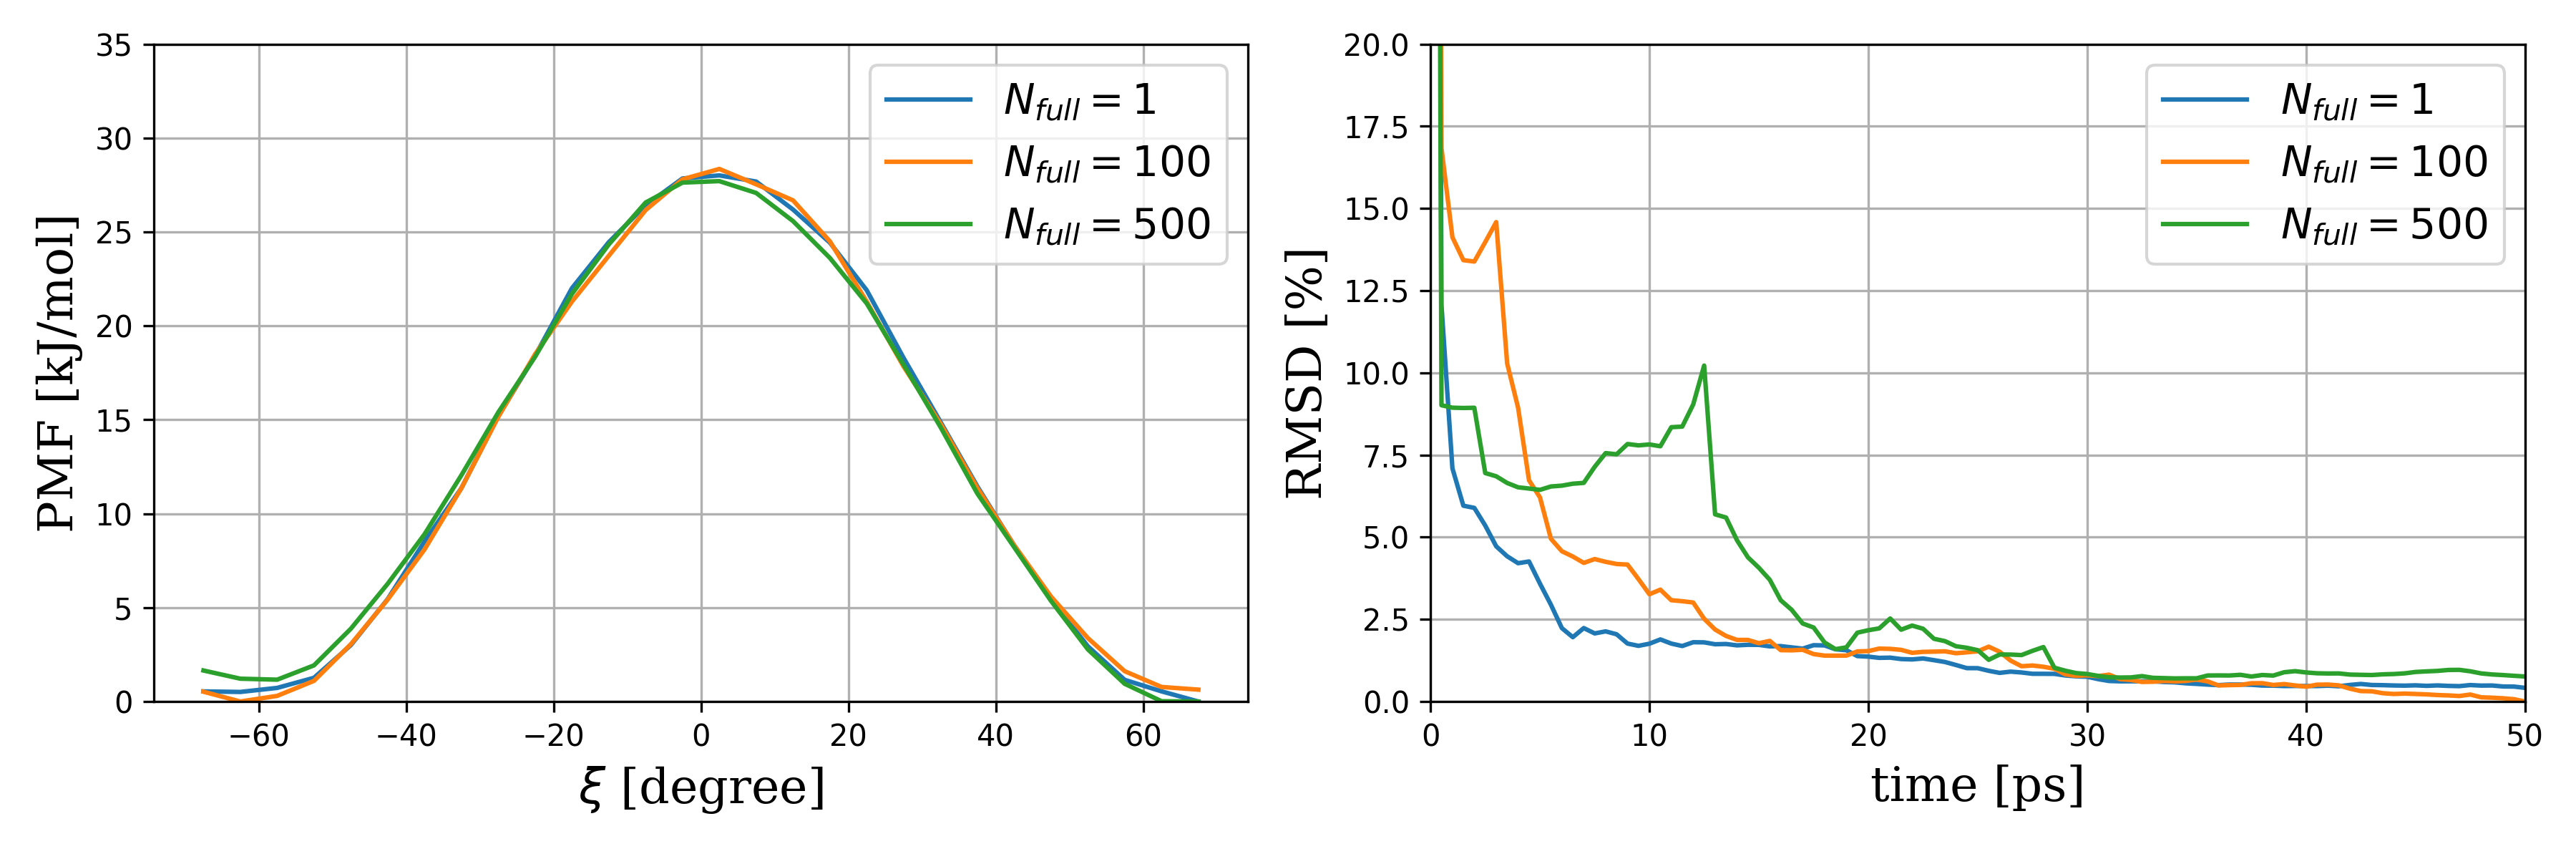
\includegraphics[width=0.99\textwidth]{bilder/benchmark/ABF_benchmark_nfull}
    \caption{Results of ABF calculations for the torsion of Cl-F-ethane for different values of $N_{full}$. Each PMF was obtained from a single 50~ps trajectory. Panels show the number of counts per bin after 50~ps, the resulting PMFs, the convergence of the PMF RMSD and the convergence of $\Delta A$, respectively. The RMSD is calculated in reference to the $N_{full}=100$ result. To calculate $\Delta A$ the probability density is integrated over both thermodynamic states. For this purpose states are separated at the maximum of the PMF.}
    \label{fig:ABF benchmark}
\end{figure}
Free energy differences $\Delta A$ are especially sensitive to small changes of the PMF in the transition state region. Because both thermodynamic states are separated at the maximum of the PMF, large changes of $\Delta A$ can occur if the maximum shifts to another bin.
This is also a result of the relatively big bin width of 5$^\circ$ applied in this test calculations.
Overall $N_{full}=100$ gives a good compromise between fast and stable convergence of the PMF as well as already nearly optimal accuracy of $\Delta A$ in the intermediate regime (20-30~ps).
However, this is only true for a small gas-phase system as this one.
For bigger systems with slow orthogonal degrees of freedom, that are not well-captured by the CV, much bigger values of $N_{full}$ might be necessary.\autocite{comer2015adaptive}
Additionally as instantaneous force samples depend on all molecular coordinates, fluctuations in estimates of the mean force grow with the system size.\autocite{alrachid2015long}

In eABF calculations the ramp function has a vary similar influence.\autocite{lesage2017smoothed}
However, mean square fluctuations $\sigma_F$ of force samples only depend on the coupling to the fictitious particle and are inversely proportional to the thermal width $\sigma_\lambda$
\begin{equation}
    \sigma_F^2 \propto \frac{1}{\beta\sigma_\lambda}
\end{equation}
At the same time CZAR offers robust estimation of the free energy gradient for a wide range of choices of $\sigma_\lambda$.\autocite{lesage2017smoothed}
The choice of $\sigma_\lambda$ is therefore a trade-off between enhanced sampling of the CV by tight coupling to $\lambda$ and estimation of the mean force with low variance.
Figure~\ref{fig:conf eABF sig} shows both limiting cases.
With a small $\sigma_\lambda$ of $1^\circ$ convergence is hindered by strong fluctuations of the mean force.
On the other hand if coupling of the fictitious particle ($\xi_\lambda=20^\circ$) is too loose, enhanced sampling of $\lambda$ leaves some metastability in $\xi$.
For $\sigma_\lambda=5^\circ$ the noise in the force estimate is reduced significantly and both thermodynamic states are sampled uniformly.
However, relatively large deviation of the PMF to the ABF result in the transition state region and a estimated free energy difference of 2~kJ/mol indicate that the simulation is not fully converged.
\begin{figure}[H]
  \centering
    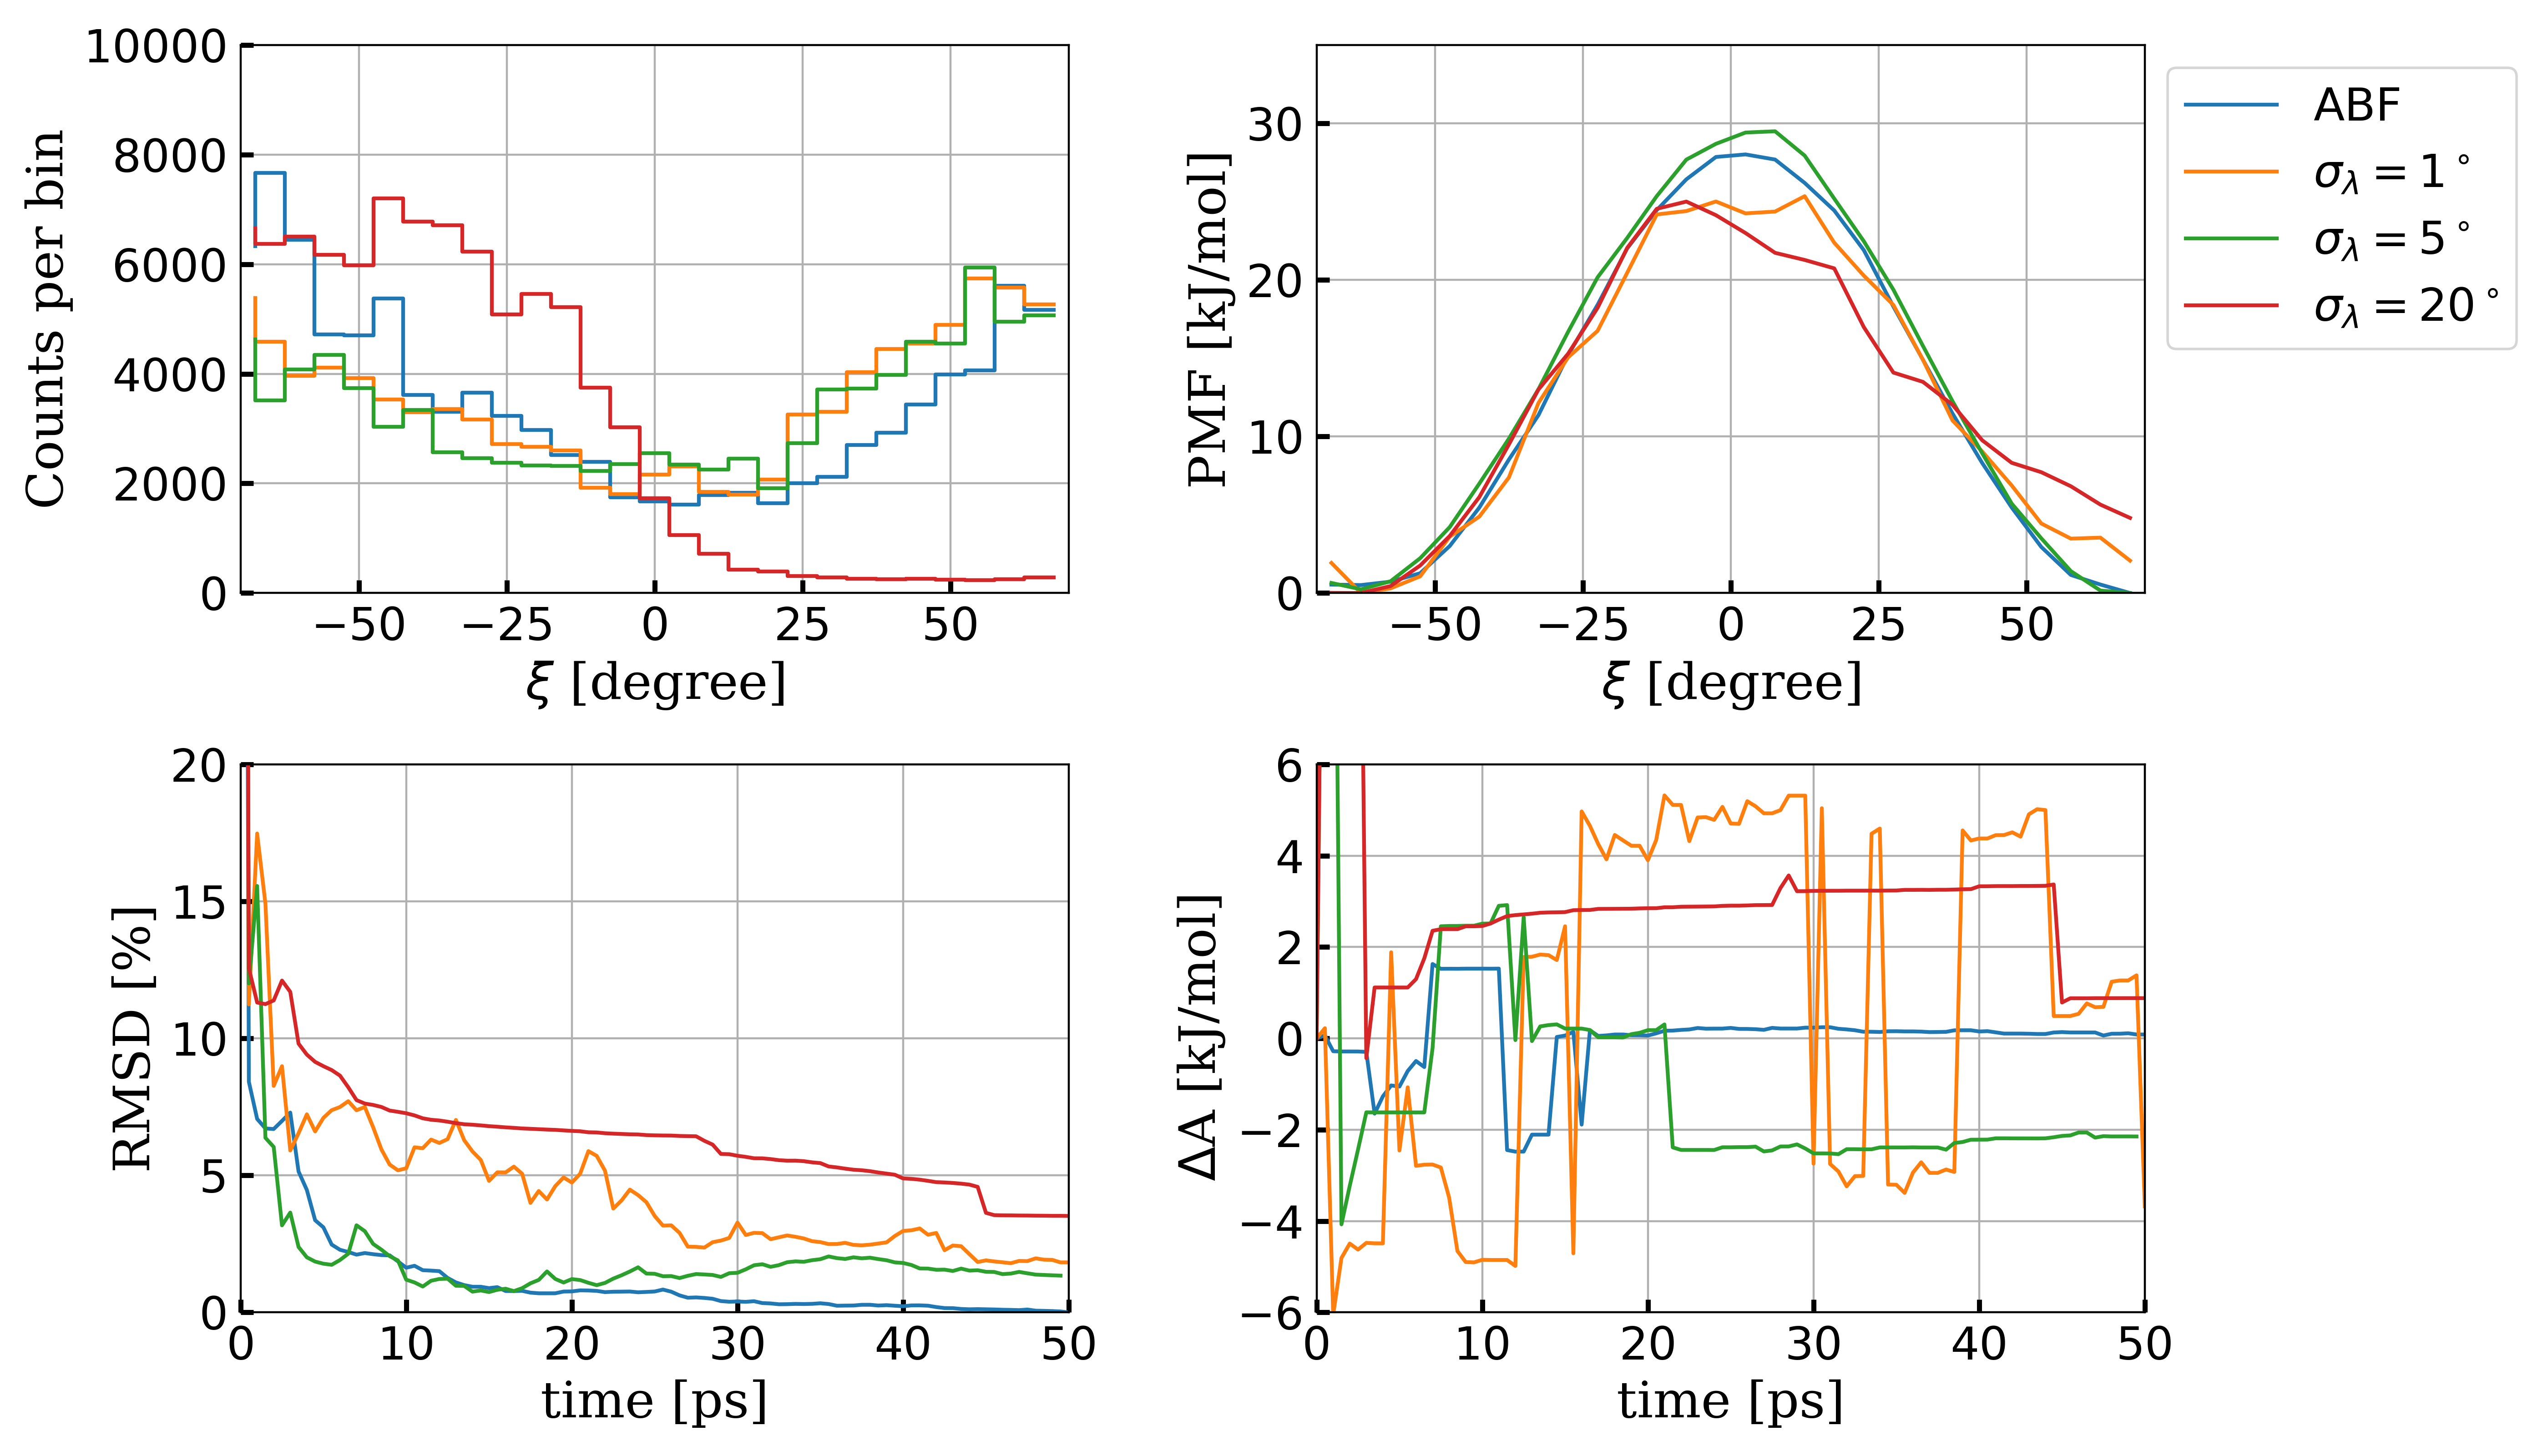
\includegraphics[width=0.99\textwidth]{bilder/benchmark/eABF_benchmark_sigma}
   \caption{
   Results of eABF/CZAR calculations for the torsion of Cl-F-ethane for different values of $\sigma_{\lambda}$. Each PMF was obtained from a single 50~ps trajectory. Panels show the number of counts per bin after 50~ps, the resulting PMFs, the convergence of the PMF RMSD and the convergence of $\Delta A$, respectively. The RMSD is calculated in reference to the ABF ($N_{full}=100$) result. To calculate $\Delta A$ the probability density is integrated over both thermodynamic states. For this purpose states are separated at the maximum of the PMF. $m_\lambda$ and $N_{full}$ are fixed to 15~a.u. and 100 samples, respectively.
   }
   \label{fig:conf eABF sig}
\end{figure}
Figure~\ref{fig:conf eABF m} shows the influence of the mass of the fictitious particle $m_\lambda$ on eABF simulations.
Similar to $N_{full}$ $m_\lambda$ has no significant impact on the resulting PMF, but influences the convergence rate of the PMF.
For bigger values of $m_\lambda$ sampling of the reaction coordinate is more uniform.
This is due to the increasing inertia of the fictitious particle, by which the overall dynamic of $\xi$ is more determined by the dynamic of $\lambda$.
For extremely high masses the inertia of the fictitious particle will slow down diffusion along the reaction coordinate, an effect that is not yet encountered with $m_\lambda=50$~a.u.
Relatively large scattering in the final estimates of $\Delta A$ from $-2$~kJ/mol to $2$~kJ/mol indicate that full convergence is close, but not yet reached in all cases.
\begin{figure}[H]
  \centering
    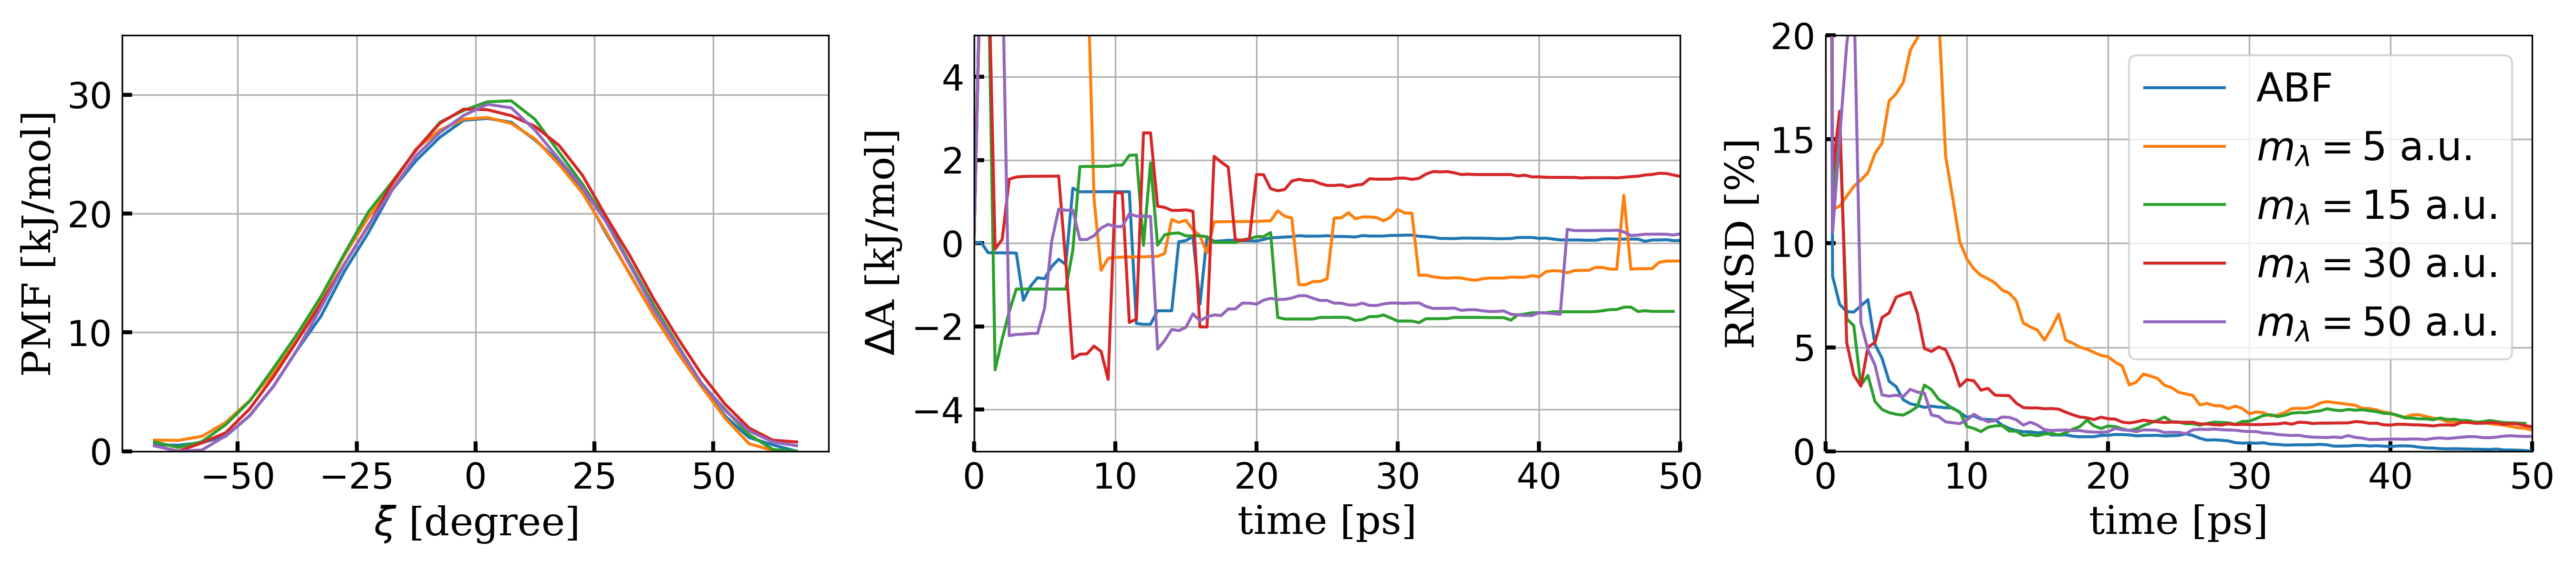
\includegraphics[width=0.99\textwidth]{bilder/benchmark/eABF_benchmark_mass}
   \caption{
     Results of eABF/CZAR calculations for the torsion of Cl-F-ethane for different values of $m_{\lambda}$. Each PMF was obtained from a single 50~ps trajectory. Panels show the number of counts per bin after 50~ps, the resulting PMFs, the convergence of the PMF RMSD and the convergence of $\Delta A$, respectively. The RMSD is calculated in reference to the ABF ($N_{full}=100$) result. To calculate $\Delta A$ the probability density is integrated over both thermodynamic states. For this purpose states are separated at the maximum of the PMF. $\sigma_\lambda$ and $N_{full}$ are fixed to $5^\circ$ and 100 samples, respectively.
   }
   \label{fig:conf eABF m}
\end{figure}
Turning to WTM-eABF leads to significant improvement of the convergence of the PMF compared to eABF, as shown in figure~\ref{fig:conf meABF}.
The incorporation of a repulsive WTM potential increases transitions of trajectories between both states and enables uniform sampling of the reaction coordinate from the beginning.
This results in faster convergence of the PMF especially in the transition state region.
For all WTM-eABF simulations the final RMSD of the PMF to the ABF result is below 1~\% and $\Delta A$ converges safely to 0~kJ/mol.
As the free energy curves are obtained from CZAR and independent of the WTM potential, the choice of parameters has no significant influence on the obtained PMF.
Also by using the well-tempered variant of the metadynamics potential, the Gaussian height is scaled down over time and converges towards the same limiting value for all initial choices of $W$.
Non-equilibrium effects are therefore less severe than with conventional metadynamics and do not prevent convergence even for high choices of $W$ in this particular example.
WTM-eABF is also less sensitive to bad choices of eABF parameters $m_\lambda$ and $N_{full}$, because slow diffusion to another thermodynamic state by too large a choice of $N_{full}$ or too small a choice of $m_\lambda$ is compensated by the WTM potential.
\begin{figure}[H]
  \centering
    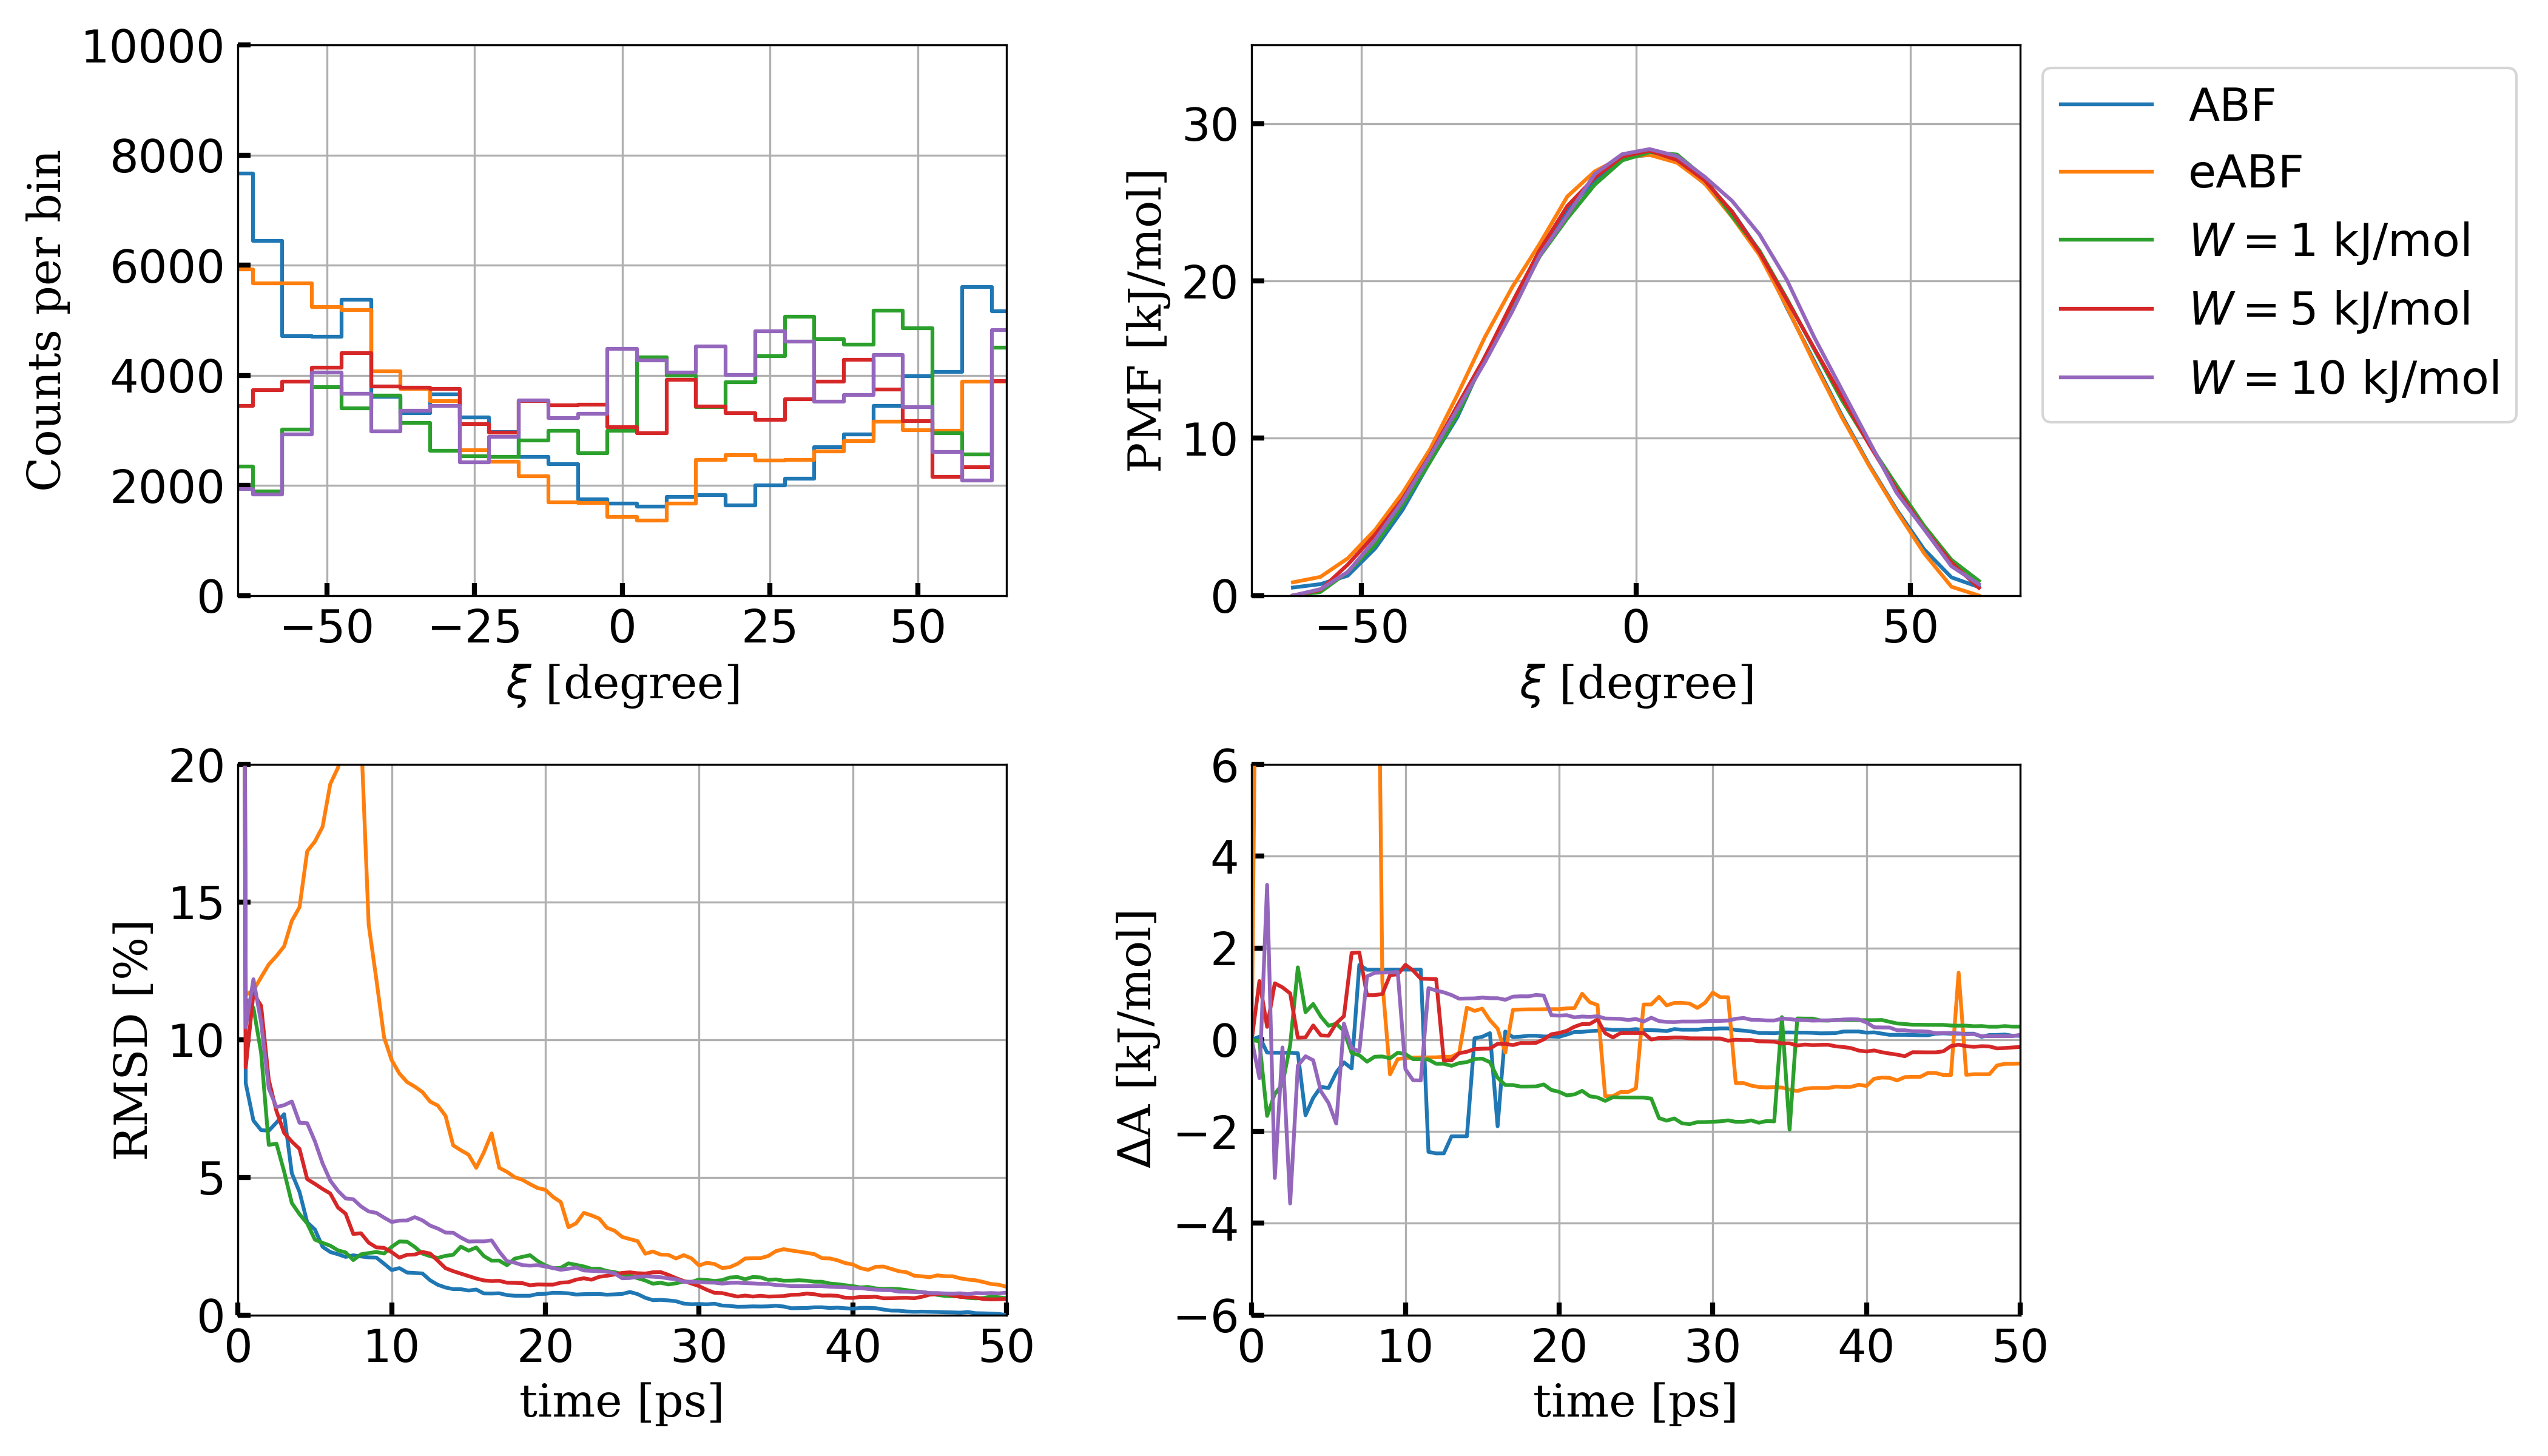
\includegraphics[width=0.99\textwidth]{bilder/benchmark/meta_eABF_benchmark}
   \caption{
    Results of WTM-eABF/CZAR calculations for the torsion of Cl-F-ethane for different values of $W$. Each PMF was obtained from a single 50~ps trajectory. Panels show the number of counts per bin after 50~ps, the resulting PMFs, the convergence of the PMF RMSD and the convergence of $\Delta A$, respectively. The RMSD is calculated in reference to the ABF ($N_{full}=100$) result. To calculate $\Delta A$ the probability density is integrated over both thermodynamic states. For this purpose states are separated at the maximum of the PMF.
    Values of $m_{\lambda}$, $\sigma_\lambda$, $N_{full}$, $\tau_G$ and $\Delta T$ are fixed at 5~a.u., $5^\circ$, 100 samples, 10~fs and 2000~K, respectively.
   }
   \label{fig:conf meABF}
\end{figure}
Until now PMFs were only calculated from single trajectories.
However, for the application of adaptive biasing methods to complex reactions scalable speedup by parallelisation is crucial.
Figure~\ref{fig:conf ABF} shows initial convergence rates for the parallelisation to two walkers by three different strategies (independent sampling, shared bias and stratification).
For ABF all strategies increase the convergence significantly.
Using a shared-bias scheme has no advantage compared to the calculation of separat trajectories in the first 6~ps, but afterwards small benefits do become noticeable, when walkers encounter pre-existing force estimates after transition to the other state and diffusive behavior sets in.
For eABF and WTM-eABF this benefits are bigger, because transition to the other state is faster.
High PMF RMSDs for the single trajectory calculations with eABF and WTM-eABF are mostly caused by inaccurate force estimates in individual bins.
As the second trajectory has not added any force samples to this area the RMSD is not improved with independent second trajectories in this cases.

To test the stratification strategy the PMF is separated to two windows, ranging from -70$^\circ$ to 0$^\circ$ and 0$^\circ$ to 70$^\circ$.
At the beginning RMSDs are higher than with single trajectories because the connection of both windows introduces large errors in the first few picoseconds.
However, confining each simulation to one state enforces uniform sampling of the reaction coordinate, which benefits convergence of the PMF.
Because metastability is no concern for this simulations, the WTM-potential has only little impact on the overall convergence rate.
Small disturbances of the system from thermal equilibrium at the beginning even slightly hindered the initial convergence rate compared to eABF.
\begin{figure}[H]
  \centering
    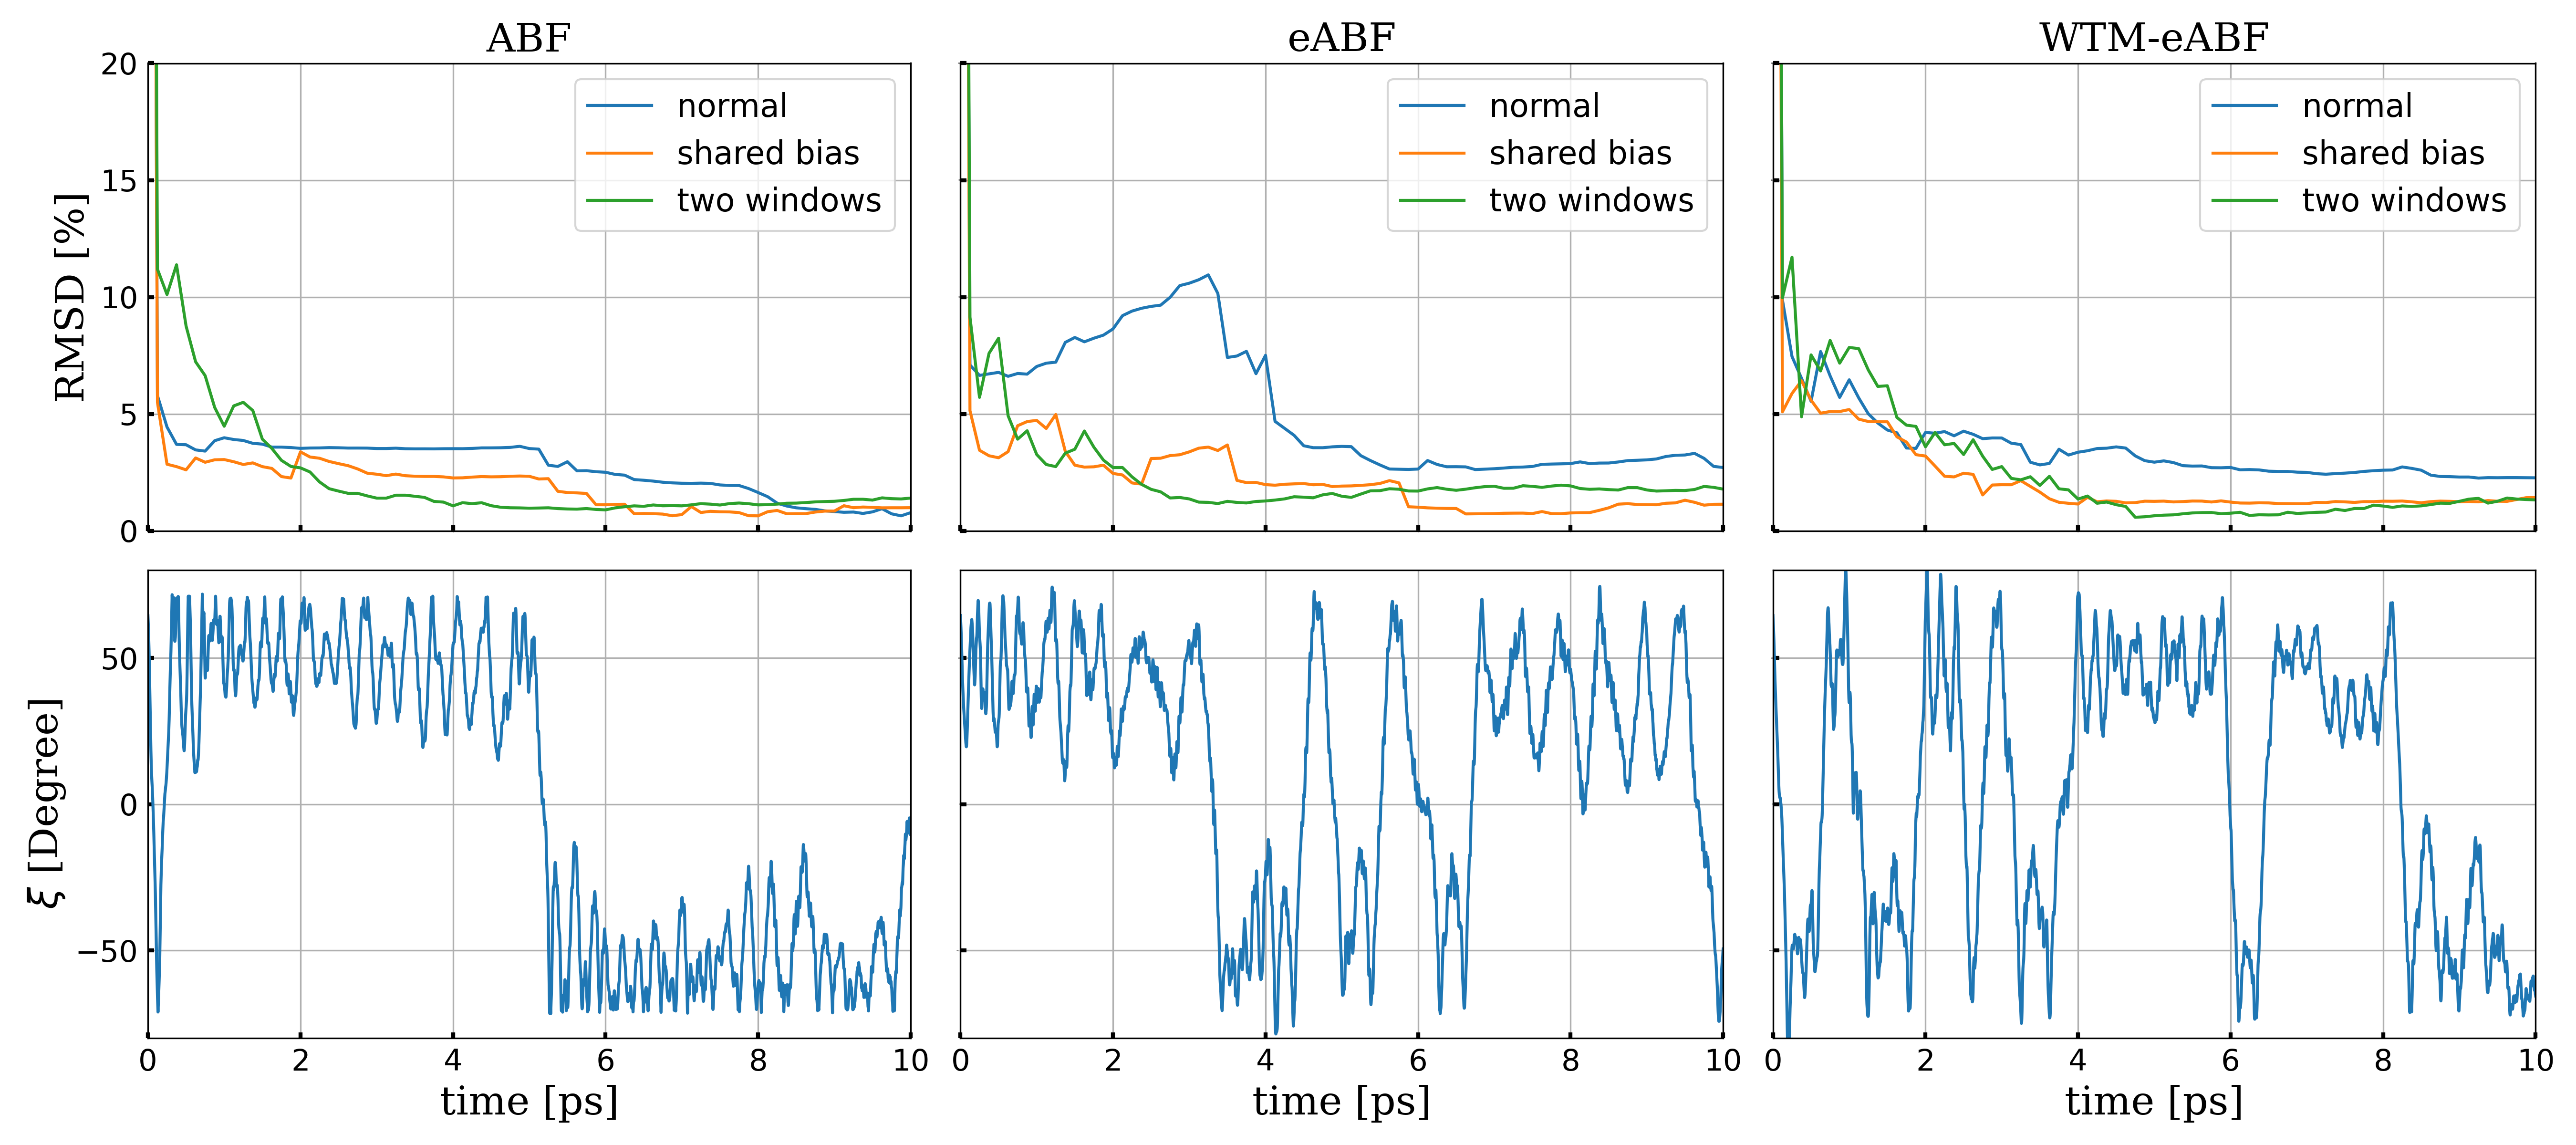
\includegraphics[width=0.85\textwidth]{bilder/benchmark/ABF_acc_benchmark}
   \caption{
   Convergence of adaptive biasing force methods with different parallelisation strategies (separate calculation of two trajectories, shared-bias-ABF and stratification to two windows of equal size). In each case one walker was started in the product and one in the reactant state. From top to bottom results obtained with ABF, eABF and WTM-eABF are given, respectively. Panels on the left show counts per bin after the first 10~ps. Panels on the right show the convergence of the PMF RMSD in reference to a 50~ps ABF trajectory. Details are given in the table~\ref{tab:benchmark params} of the appendix.}
   \label{fig:conf ABF}
\end{figure}
Overall, all three methods converge to the same PMF within a RMSD of 1~\%.
However, free energy differences are extremely sensitive to fluctuations of the PMF at the transition state region.
This is caused by the wide bin width of 5$^\circ$ that was applied in this calculations.
By accelerating sampling of the transition state region, WTM-eABF/CZAR safely converges to the correct free energy difference for a wide range of parameters.
In the following the application of WTM-eABF/CZAR will be demonstrated for two more complicated reaction mechanisms, involving a S$_N$2 type reaction and formation of deoxyadenosine.
\newpage
\section{Illustrative Application to Reactions of Small Molecules}
\label{sec:Sn2}
To demonstrate the performance of WTM-eABF compared to Umbrella Sampling
the PMF of the an S$_N$2 type reaction was calculated with both methods.
Results are given in figure~\ref{fig:Sn2}.
\begin{figure}[H]
  \centering
    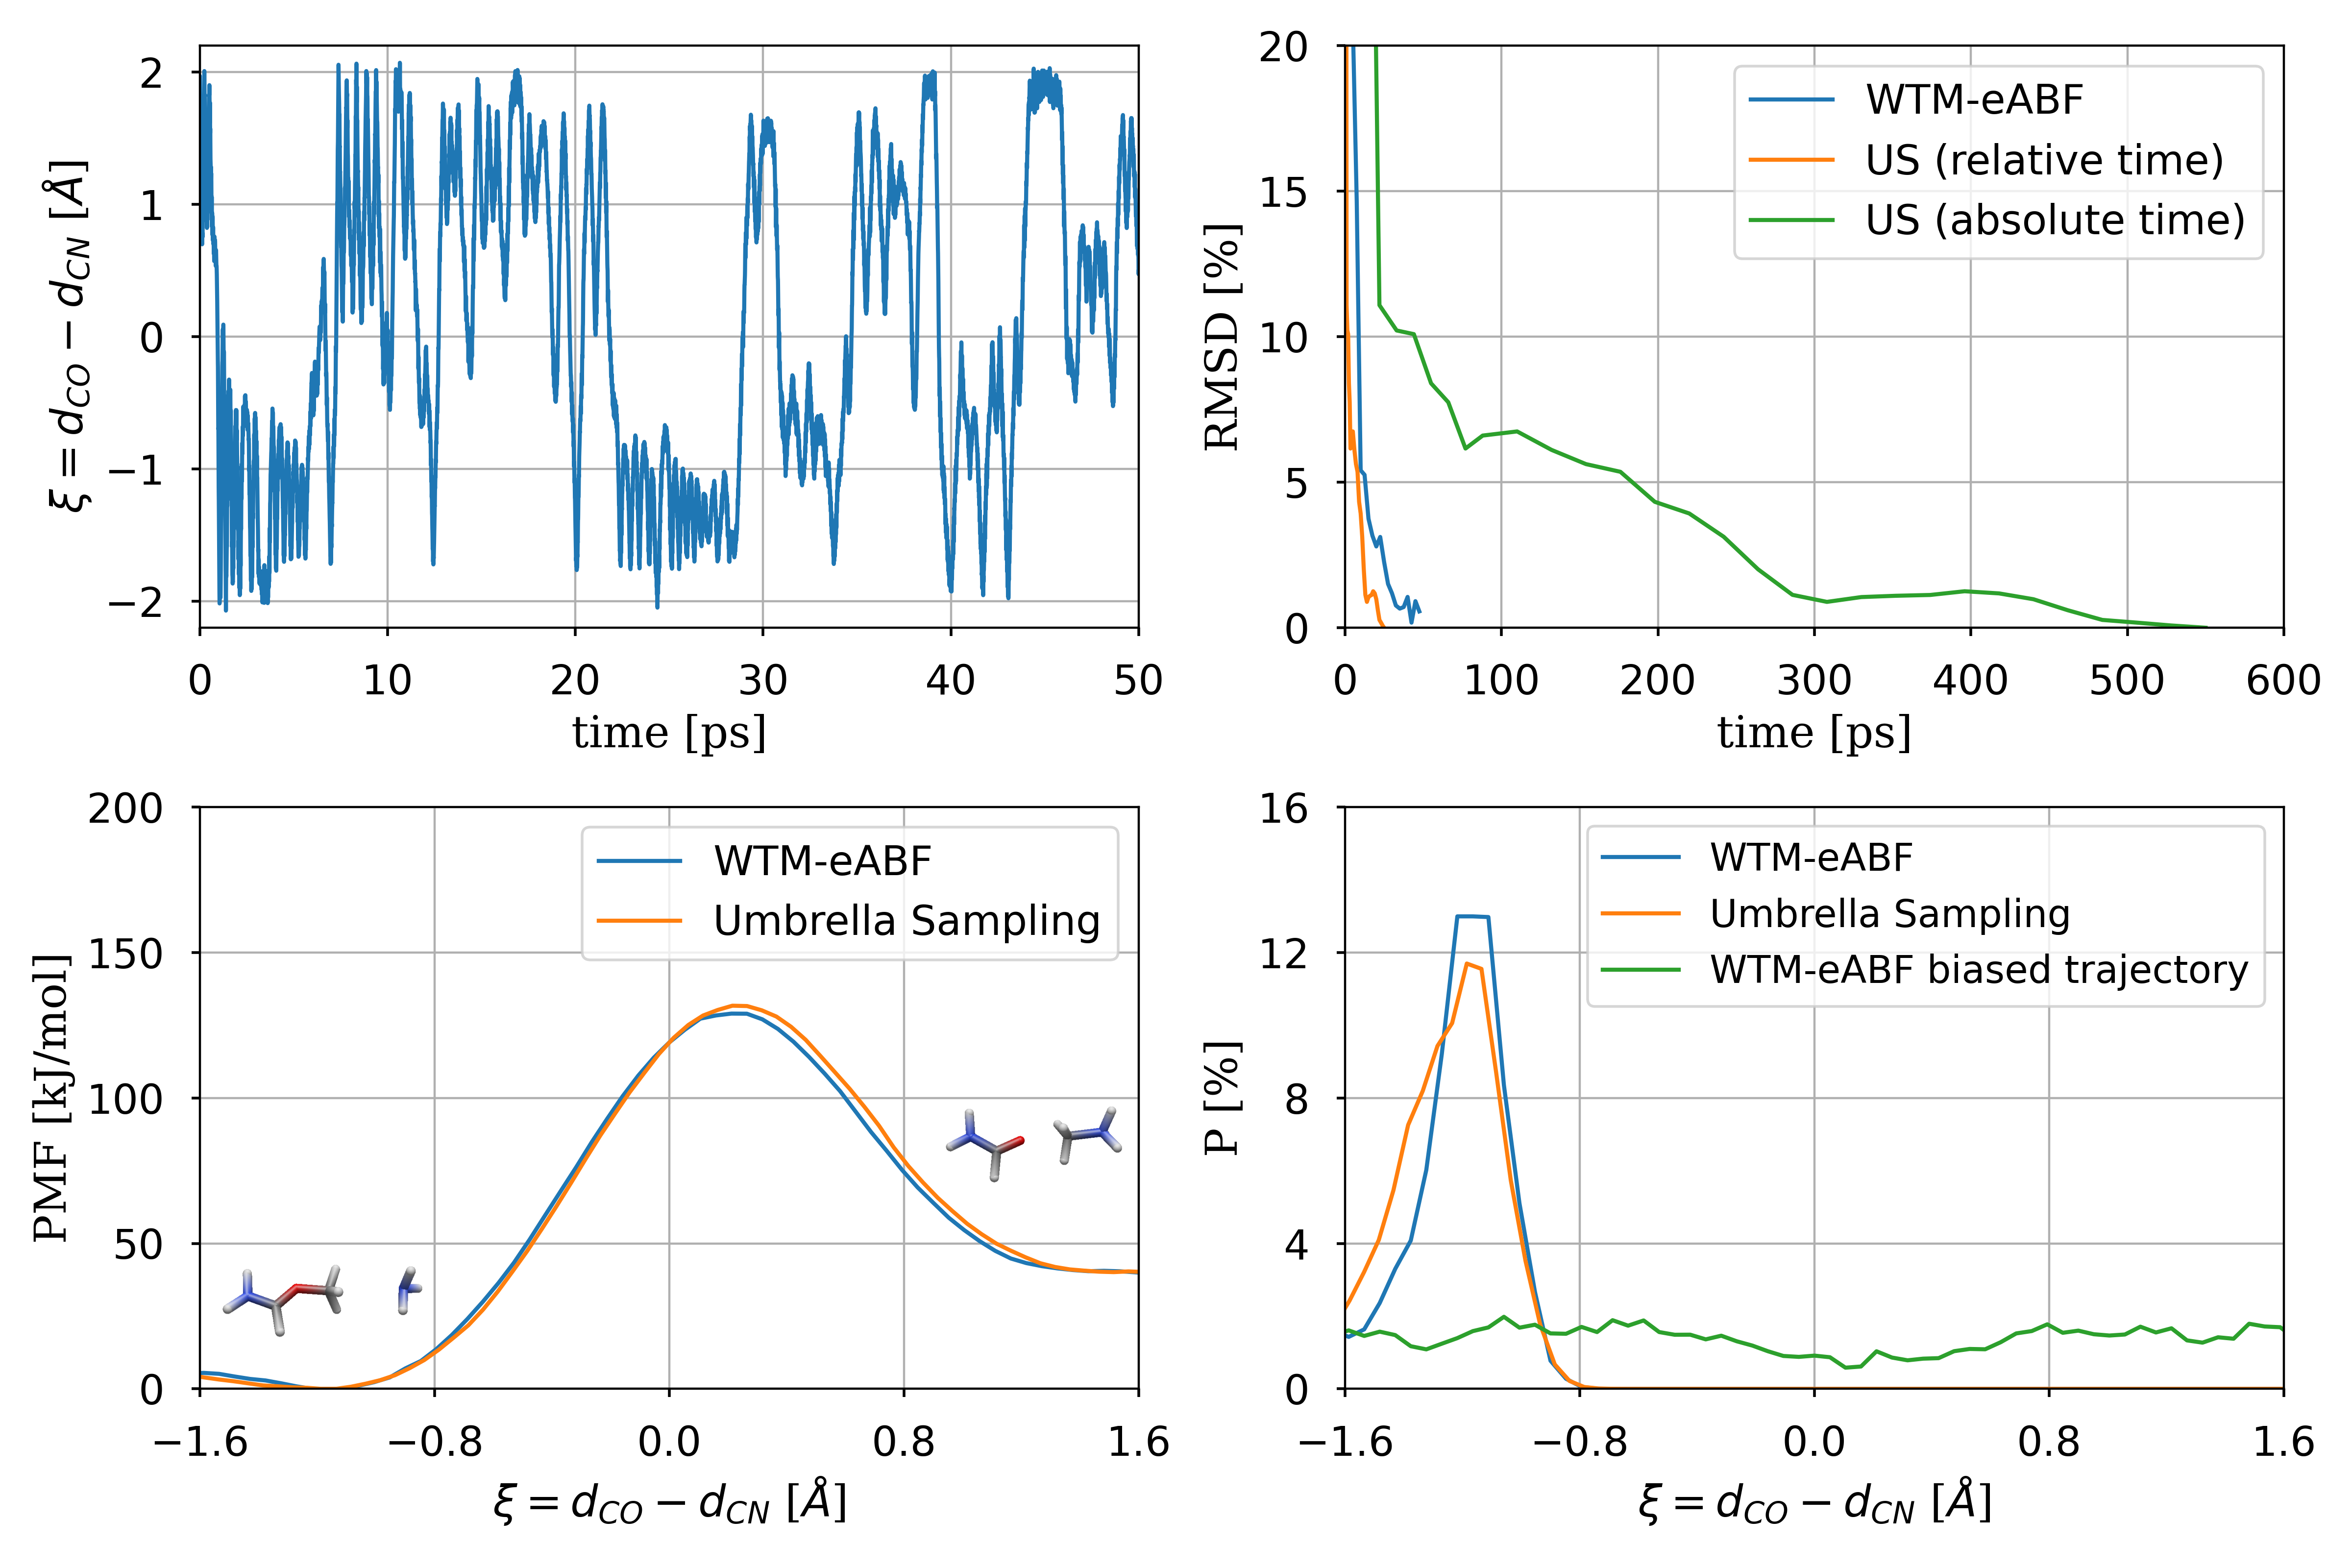
\includegraphics[width=0.999\textwidth]{bilder/sirt5_SW}
  \caption{
    Application of WTM-eABF and US to an S$_N$2 reaction. In the top left the time trajectory of the WTM-eABF simulation is shown. Umbrella Sampling was done by simulating 25~ps trajectories in 22 independent windows, which adds up to a total simulated time of 550~ps. The top right panel gives the convergence of the PMFs obtained with reference to the US result. In bottom left the PMFs obtained from US/MBAR and WTM-eABF/CZAR are shown. The bottom right panel shows corresponding probability densities together with the biased probability density of the WTM-eABF trajectory.
  }
  \label{fig:Sn2}
\end{figure}
The US PMF is reproduced by WTM-eABF in a single 50~ps trajectory with a final RMSD of 0.56~\%.
The top right panel shows the trajectory of the WTM-eABF simulation.
Uniform sampling of the hole reaction coordinate is obtained from the beginning.
The probability density of the biased simulation given in the bottom right panel is almost fully uniform.
In contrast, the strength of US lies in the massive parallelisation of sampling to multiple windows along the reaction coordinate.
However, as shown in the top right panel of figure~\ref{fig:Sn2} the convergence of Umbrella Sampling with the absolute amount of sampled data is rather poor.
In contrast WTM-eABF can reproduce the US PMF in a single 50~ps trajectory, reducing the absolute amount of sampled data by a factor of 10.

As a second example the formation of deoxyadenosine in a ring closing reactions is considered.
Figure~\ref{fig:ool results} shows the obtained PMF as well as the biased and unbiased probability distributions.
\begin{figure}[H]
  \centering
    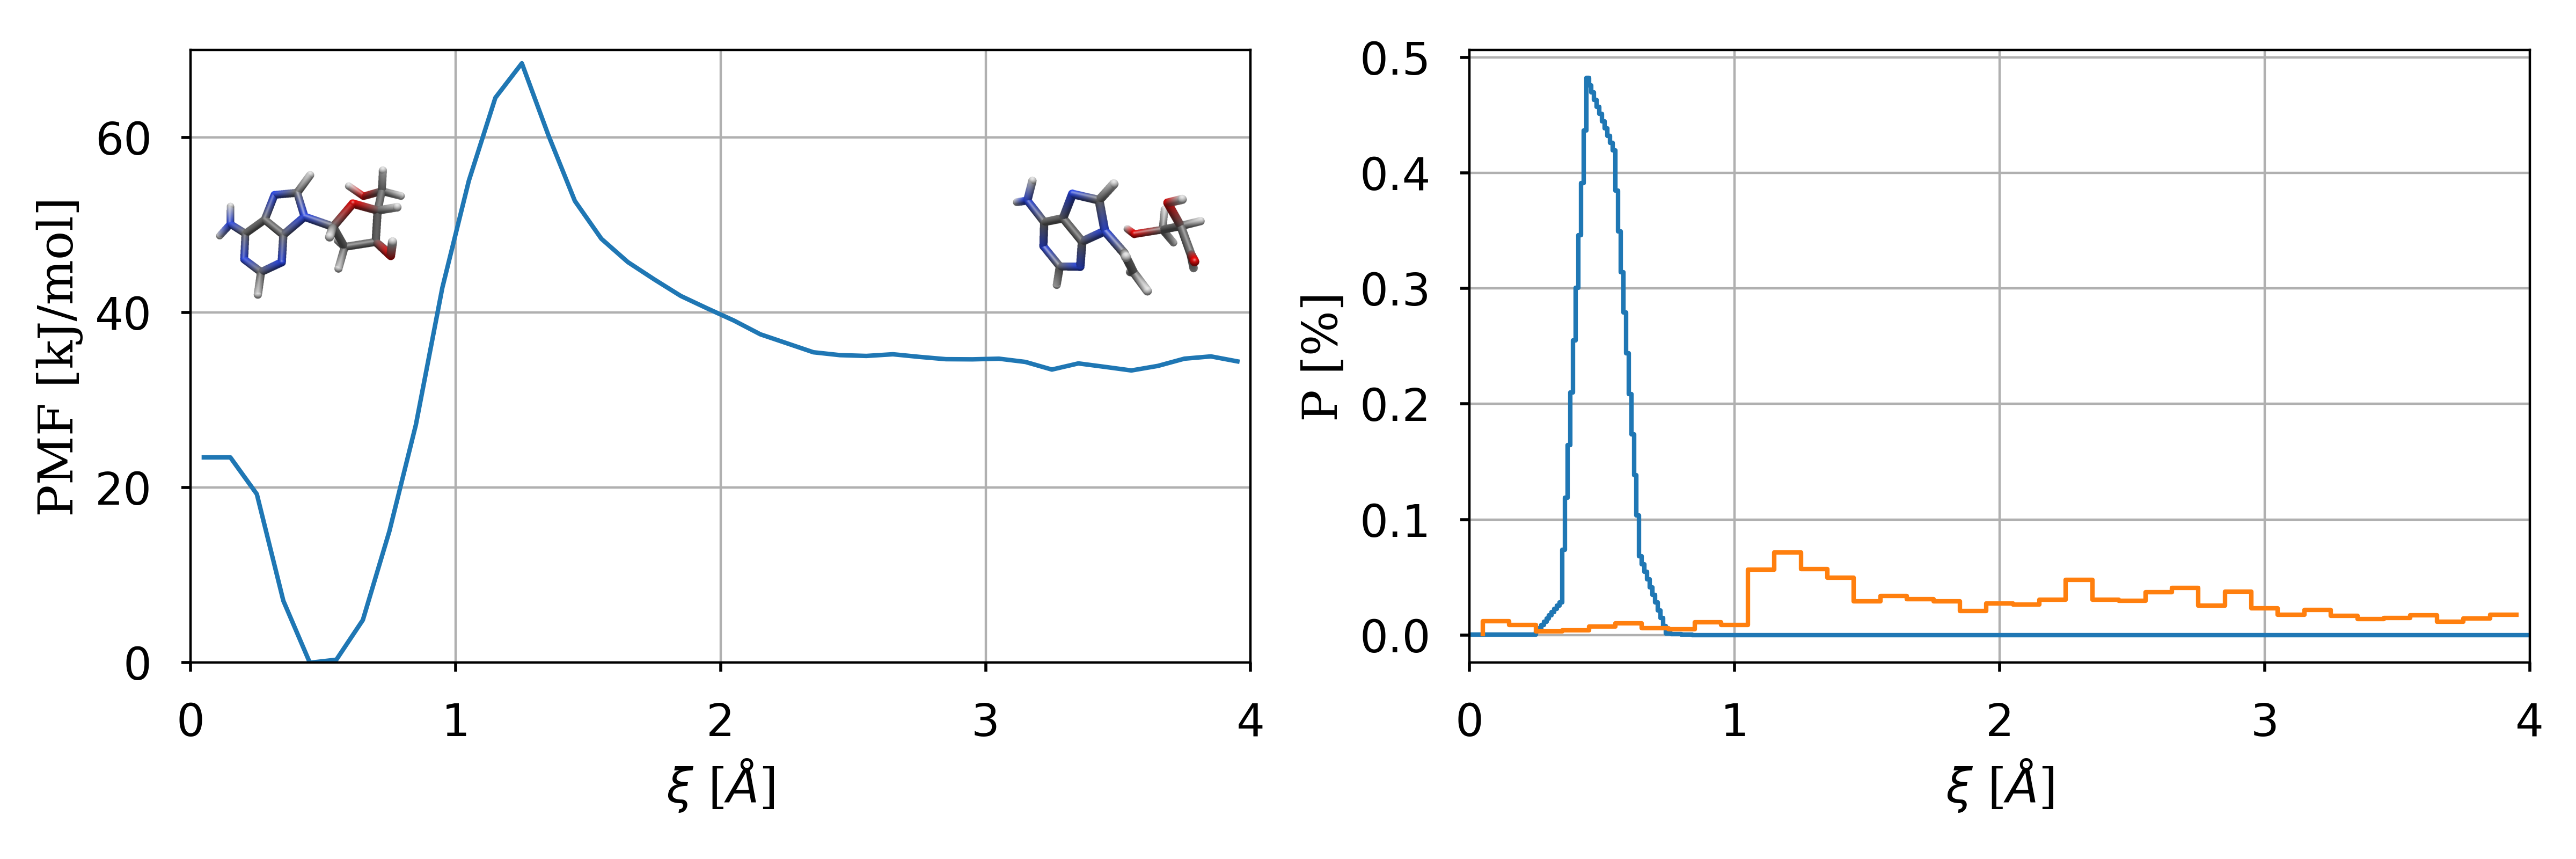
\includegraphics[width=0.999\textwidth]{bilder/ool}
  \caption{
    Application of shared bias WTM-eABF/CZAR to a ring formation reaction in deoxyadenosine. The reaction coordinate is a linear combination of four bond distances (see eq.~\ref{eq:CV ool}). Panels show the obtained PMF and the biased and unbiased probability density.
  }
  \label{fig:ool results}
\end{figure}
This particular example involves a much more complicated CV than the previous examples, consisting of the linear combination of four different bond length.
Sampling of the reaction coordinate is less uniform than before and trajectories spent less time in the product than in the educt state.
This indicates that the CV does not fully capture all slow degrees of freedom of the system, which is therefore trapped in the reactant state for a longer period of time.
Specifically, the relative stereo-chemical arrangement of the two molecules to each other represents an additional slow degree of freedom, that is not captured by the CV.
Thus transition from the product to the educt state is fully diffusive, but the backtransition is hindered.
This underlines the importance of the availability of good CVs for the application of adaptive biasing methods.
However, uniform sampling could still be enforced by stratification of the reaction coordinate to two windows, one for the reactant and one for the product state.
